\documentclass{beamer}
\usepackage{amssymb, amsfonts, latexsym, amsthm, amsmath, framed, esvect, parskip}
\usepackage{amsmath, amssymb, framed, tcolorbox, mathrsfs, xcolor, graphicx}
\usepackage{multirow, booktabs, makecell}
\usepackage[backend=biber,style=numeric,sorting=none]{biblatex}
\setbeamerfont{footnote}{size=\tiny}
\addbibresource{ref.bib}
\tcbuselibrary{theorems}
\usepackage{listings}
\definecolor{green}{rgb}{0,0.6,0}
\definecolor{gray}{rgb}{0.5,0.5,0.5}
\definecolor{mauve}{rgb}{0.58,0,0.82}
\lstset{
    frame=none,
    language=Java,
    showstringspaces=false,
    columns=fullflexible,
    basicstyle = \ttfamily\small,
    numbers=none,
    numberstyle=\tiny\color{gray},
    keywordstyle=\color{blue},
    commentstyle=\color{green},
    stringstyle=\color{mauve},
    breaklines=true,
    morekeywords={function},
    breakatwhitespace=true,
    tabsize=4
}

% Beamer theme setting
\definecolor{myteal}{cmyk}{0.5,0,0.15,0}
\usecolortheme[named=myteal]{structure}
\definecolor{my-yellow}{cmyk}{0,0.2,0.7,0,1.00}
\definecolor{my-blue}{cmyk}{0.80, 0.13, 0.14, 0.04, 1.00}
\definecolor{my-green}{cmyk}{0.4,0,0.4,0,1.00}
\tcbset{
defstyle/.style={fonttitle=\bfseries\upshape, colback=my-yellow!5,colframe=my-yellow!80!black},
theostyle/.style={fonttitle=\bfseries\upshape, colback=my-blue!5,colframe=my-blue!80!black},
corstyle/.style={fonttitle=\bfseries\upshape, colback=my-green!5,colframe=my-green!80!black},
}
\usetheme{Madrid}
\setbeamertemplate{itemize items}[triangle]
\setbeamertemplate{enumerate items}[default]

\title{Week 3 Report}
\author{Ben Chen}
\institute{Dept of Computer Science and Engineering, SUSTech}
\date{\today}

\begin{document}
\frame{\titlepage}

\begin{frame}{TOC}
\begin{table}[ht]
    \tiny
	\centering
	\begin{tabular}[c]{ccccc}
		\toprule
        Title & Conference & Institute & Authors & Idea \\
		\midrule
        \makecell{Branch History Injection: \\ On the Effectiveness of \\ Hardware Mitigations Against \\ Cross-Privilege Spectre-v2 Attacks} & USENIX '22 & VUSec & \makecell{Enrico Barberis \\ Pietro Frigo \\ Marius Muench \\ Herbert Bos \\ Cristiano Giuffrida}  & \makecell{Context-based branch \\ prediction is not isolated, \\ which can be polluted \\ by attacker.} \\ \\ 
        \makecell{TIKTAG: Breaking ARM’s \\ Memory Tagging Extension \\ with Speculative Execution} & Black Hat '24 & UOS & \makecell{Juhee Kim et al}  & \makecell{Use speculative check \\ of tag to leak the \\ check result without \\ causing fault} \\ \\ 
        \makecell{PACMAN: Attacking ARM \\ Pointer Authentication with \\ Speculative Execution} & \makecell{DEFCON 30 \\ ICCA '22} & MIT & \makecell{Joseph Ravichandran \\ Weon Taek Na \\ Jay Lang \\ Mengjia Yan} & \makecell{Speculative check to leak \\ correctness of forging a PAC \\ without causing fault} \\
		\bottomrule
	\end{tabular}
\end{table}
\end{frame}

\begin{frame}{Branch History Injection\cite{bhi}}
\begin{figure}
    \begin{center}
        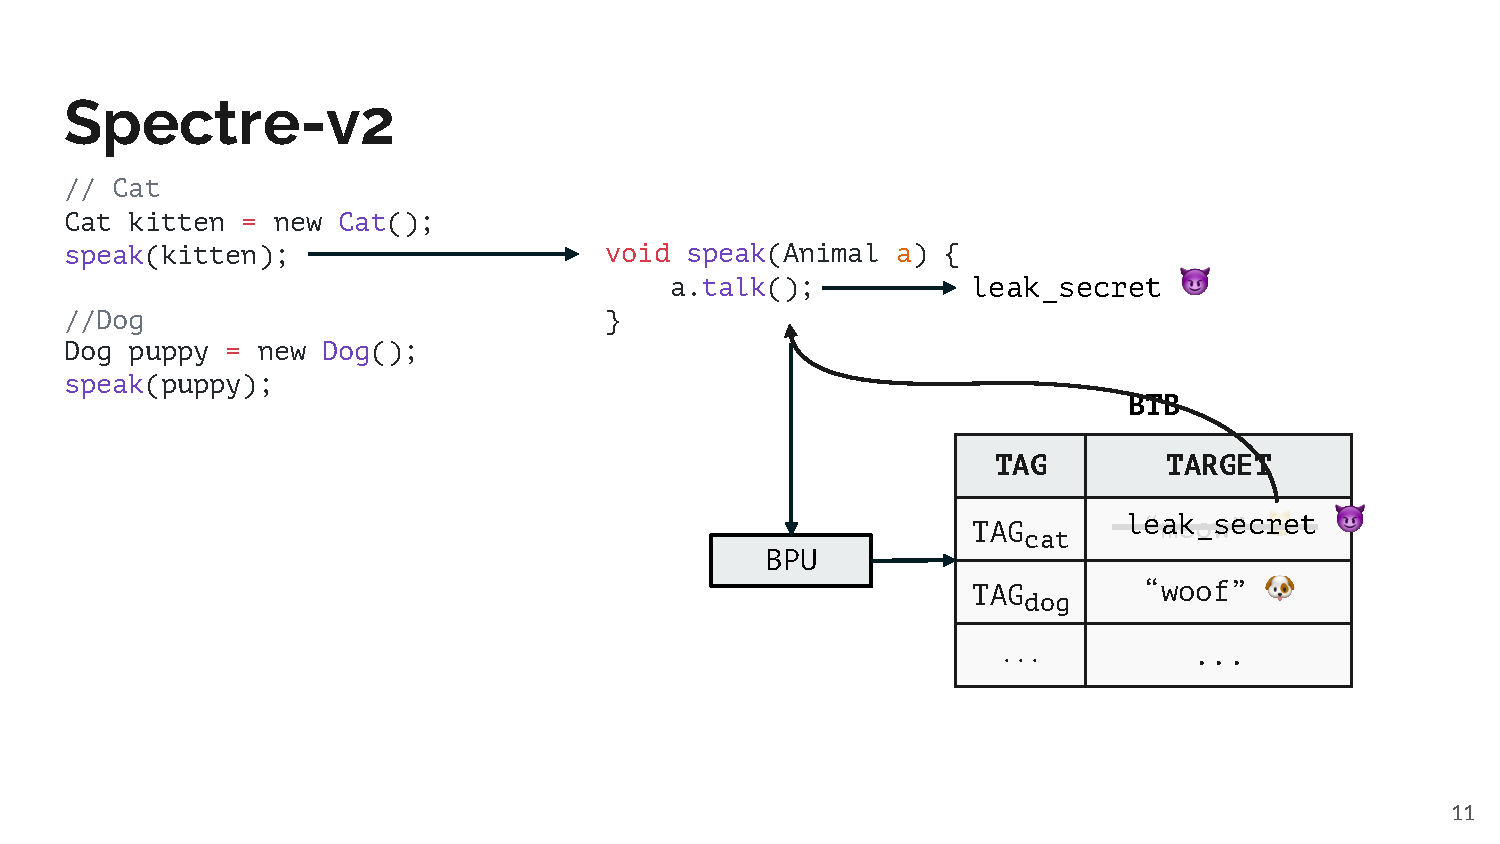
\includegraphics[width=1\textwidth]{img/spectre-v2.pdf}
    \end{center}
\end{figure}
    
\end{frame}

\begin{frame}[fragile]{Branch History Injection\cite{bhi}}
Software mitigation: Retpoline. Change the victim jump instruction \newline
\begin{lstlisting}
jmp *%r11
\end{lstlisting}

to \newline

\begin{lstlisting}
call set_up_target      (1)
capture_spec:           (4)
    pause
    jmp capture_spec
set_up_target:
    mov %r11, (%rsp)    (2)
    ret                 (3)
\end{lstlisting}

Replace attacker's target with innocuous code.
\end{frame}

\begin{frame}{Branch History Injection\cite{bhi}}
    \begin{figure}
        \begin{center}
            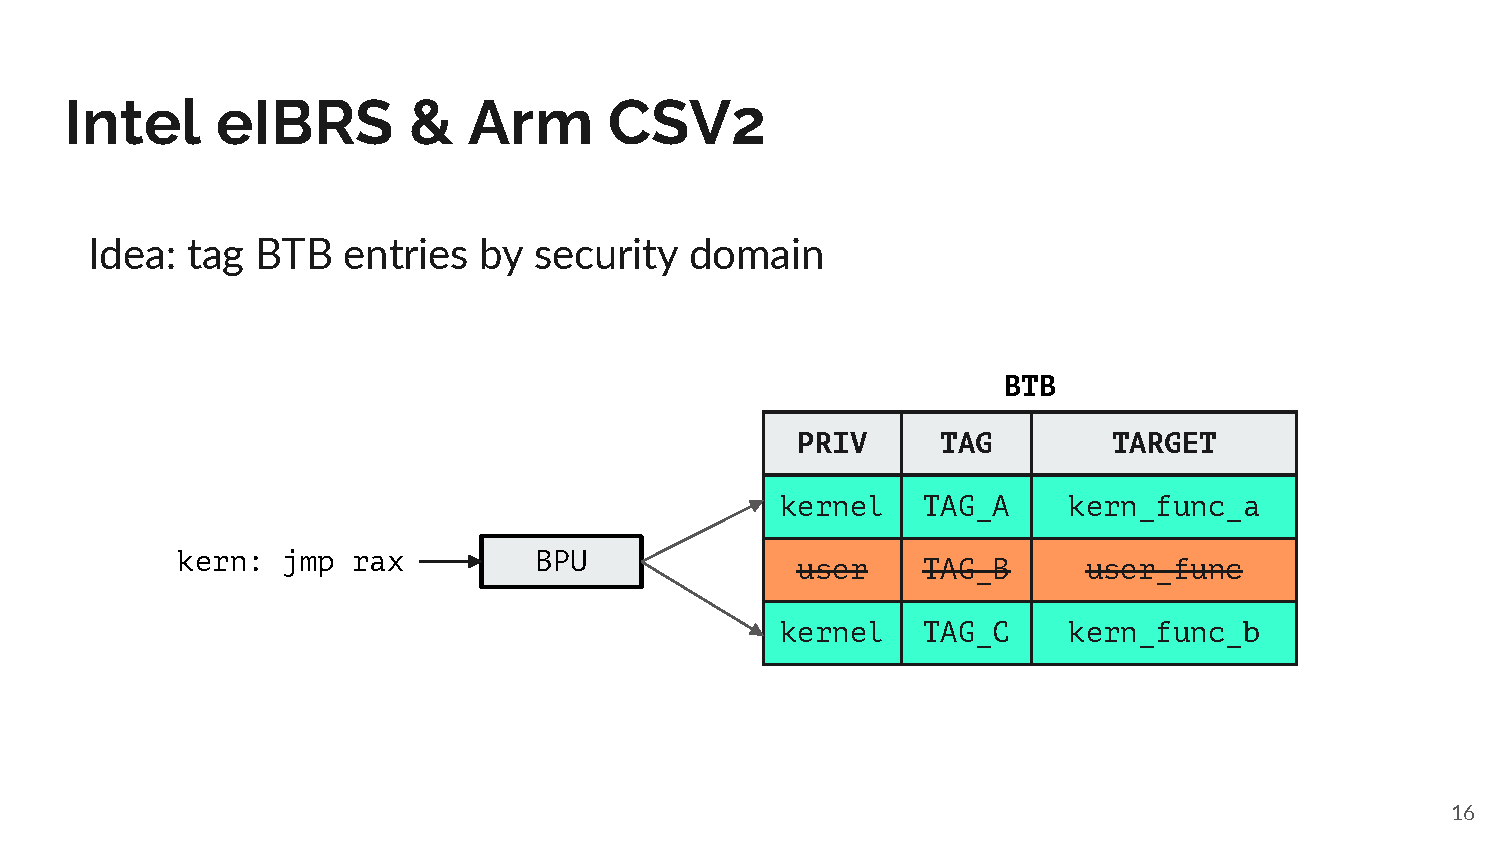
\includegraphics[width=1\textwidth]{img/elbrs.pdf}
        \end{center}
    \end{figure} 
\end{frame}

\begin{frame}{Branch History Injection\cite{bhi}}
    \begin{figure}
        \begin{center}
            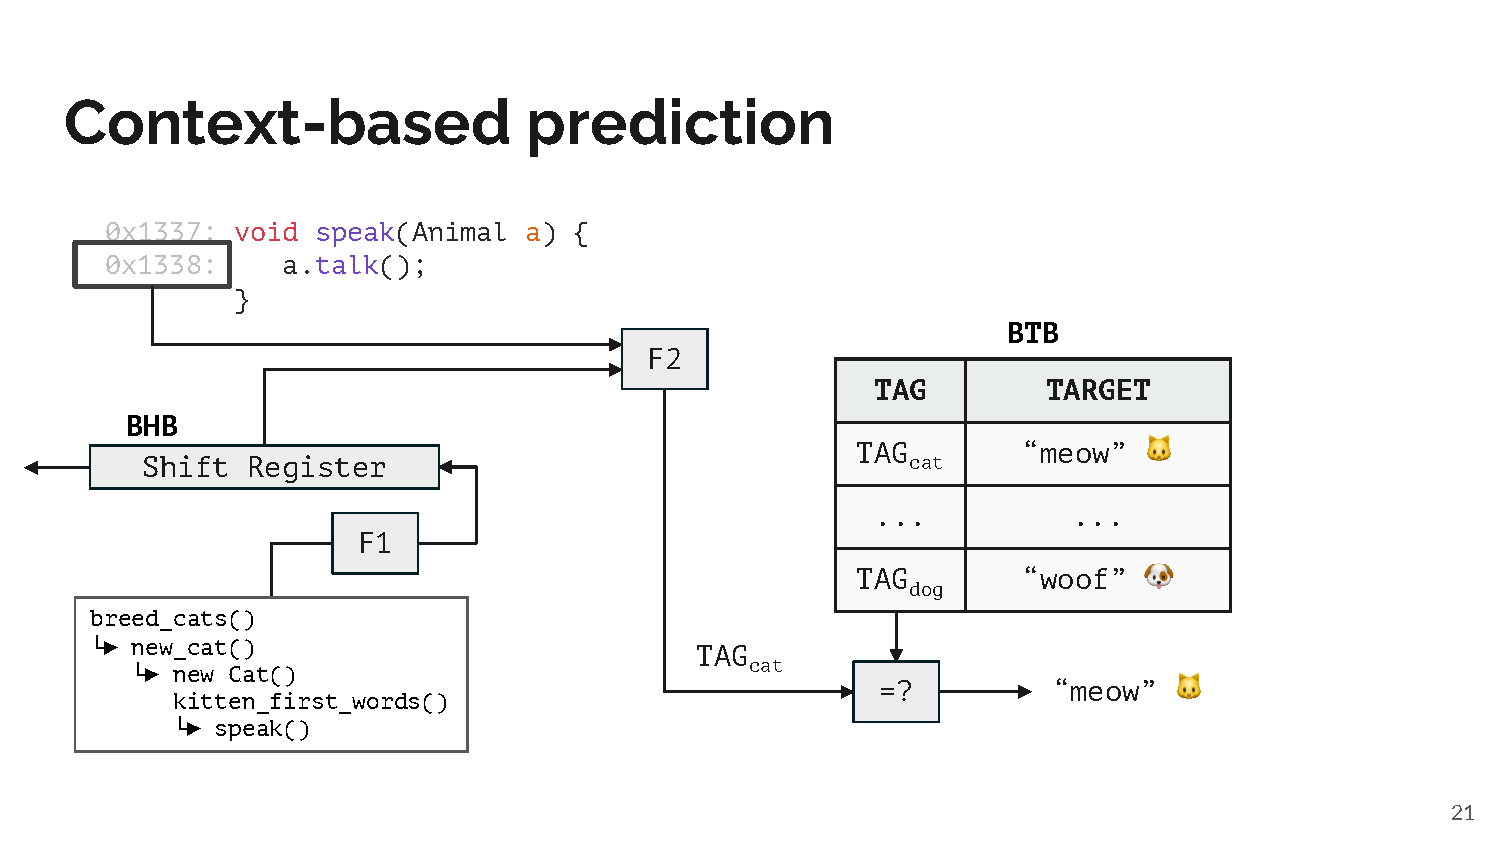
\includegraphics[width=1\textwidth]{img/context.pdf}
        \end{center}
    \end{figure} 
\end{frame}

\begin{frame}{Branch History Injection\cite{bhi}}
    \begin{figure}
        \begin{center}
            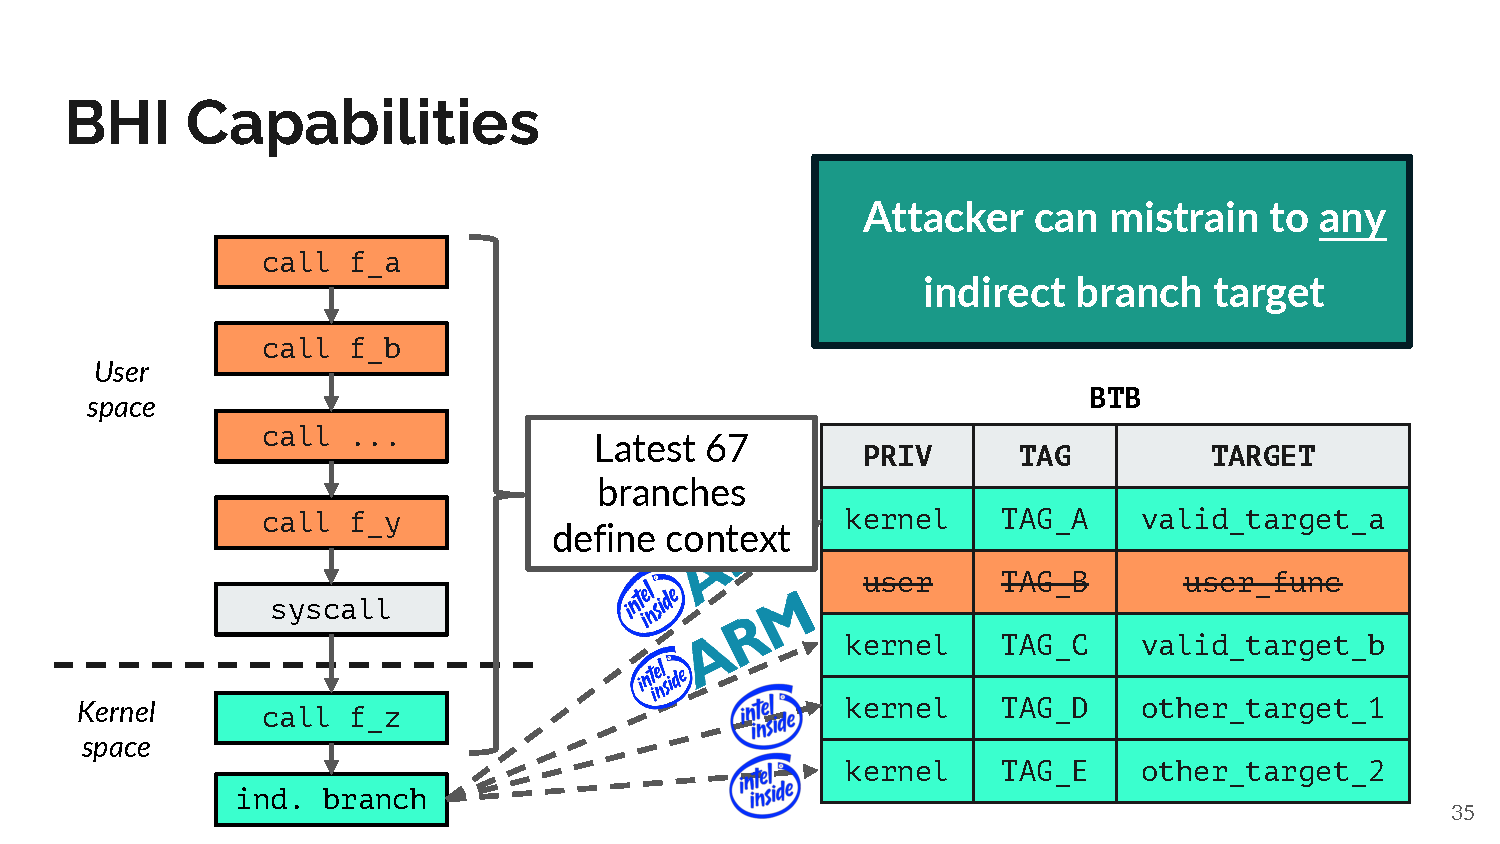
\includegraphics[width=1\textwidth]{img/capability.pdf}
        \end{center}
    \end{figure} 
\end{frame}

\begin{frame}{Branch History Injection\cite{bhi}}
    \begin{figure}
        \begin{center}
            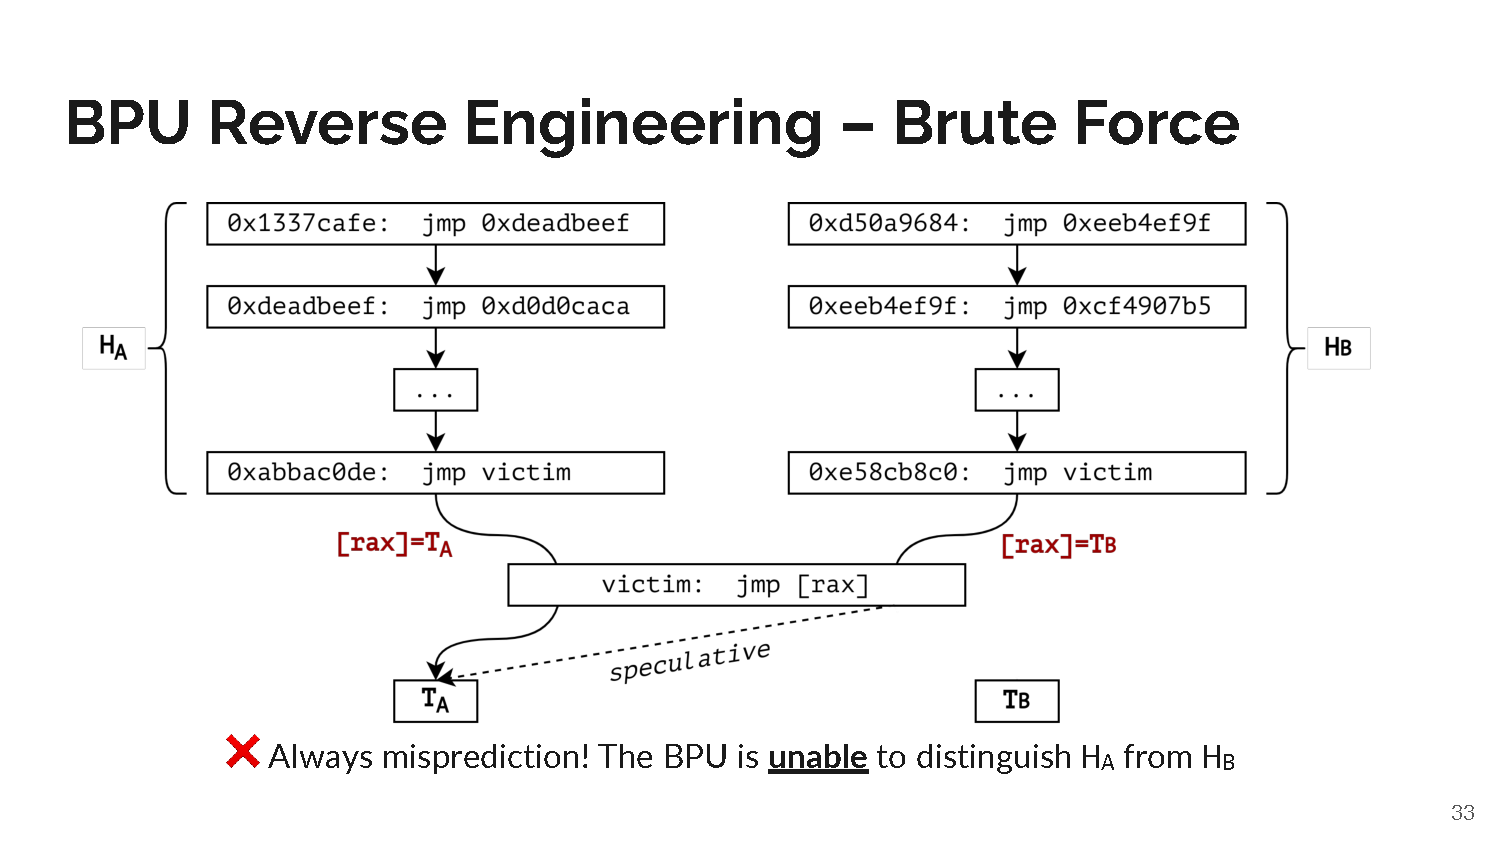
\includegraphics[width=1\textwidth]{img/bruteforce.pdf}
        \end{center}
    \end{figure} 
\end{frame}

\begin{frame}{Branch History Injection\cite{bhi}}
    \begin{figure}
        \begin{center}
            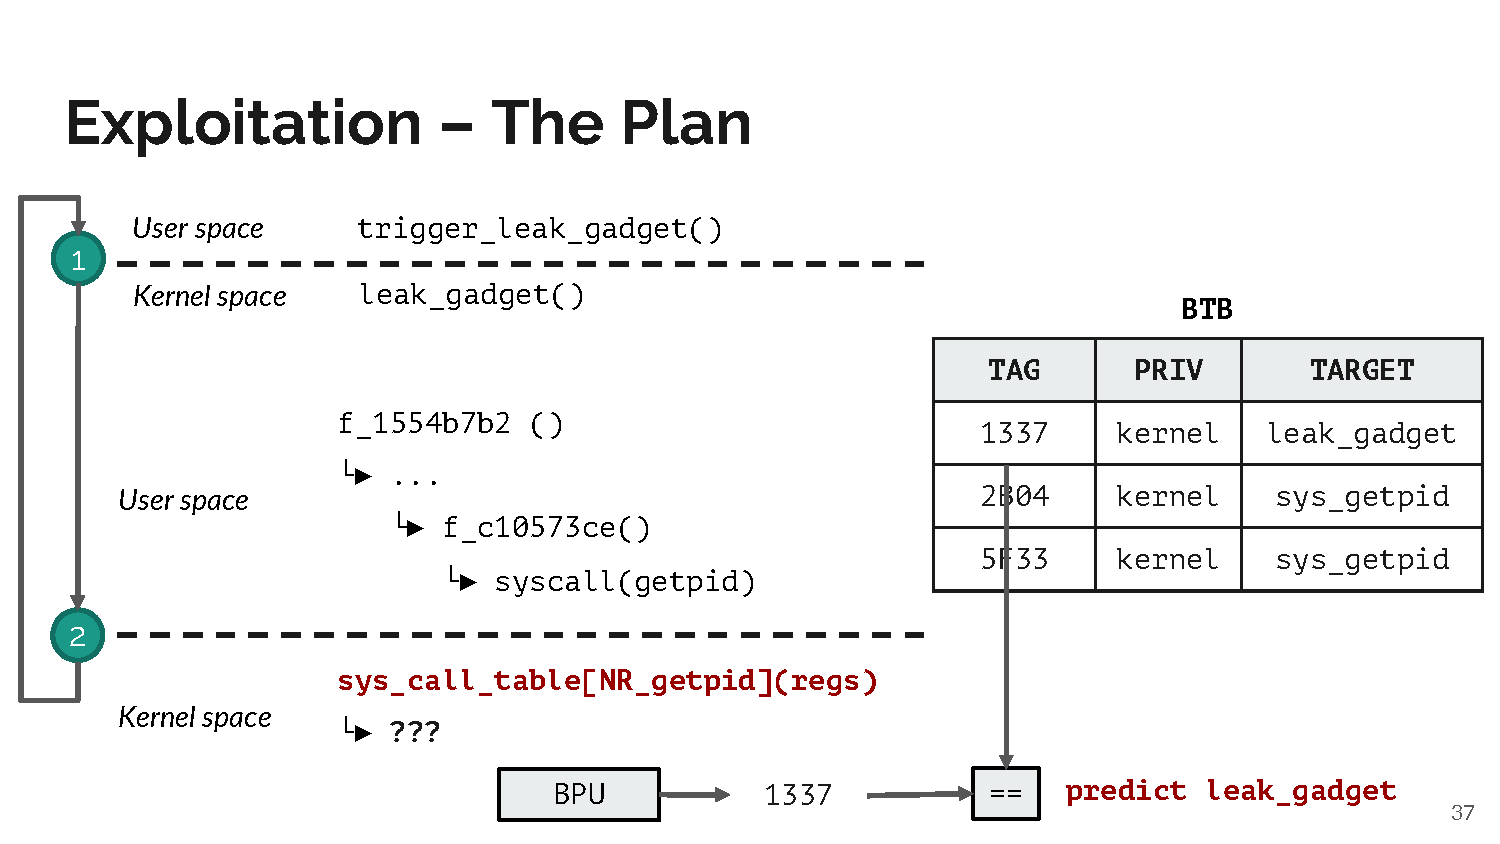
\includegraphics[width=1\textwidth]{img/exploit.pdf}
        \end{center}
    \end{figure}  
\end{frame}

\begin{frame}{Branch History Injection\cite{bhi}}
    \begin{figure}
        \begin{center}
            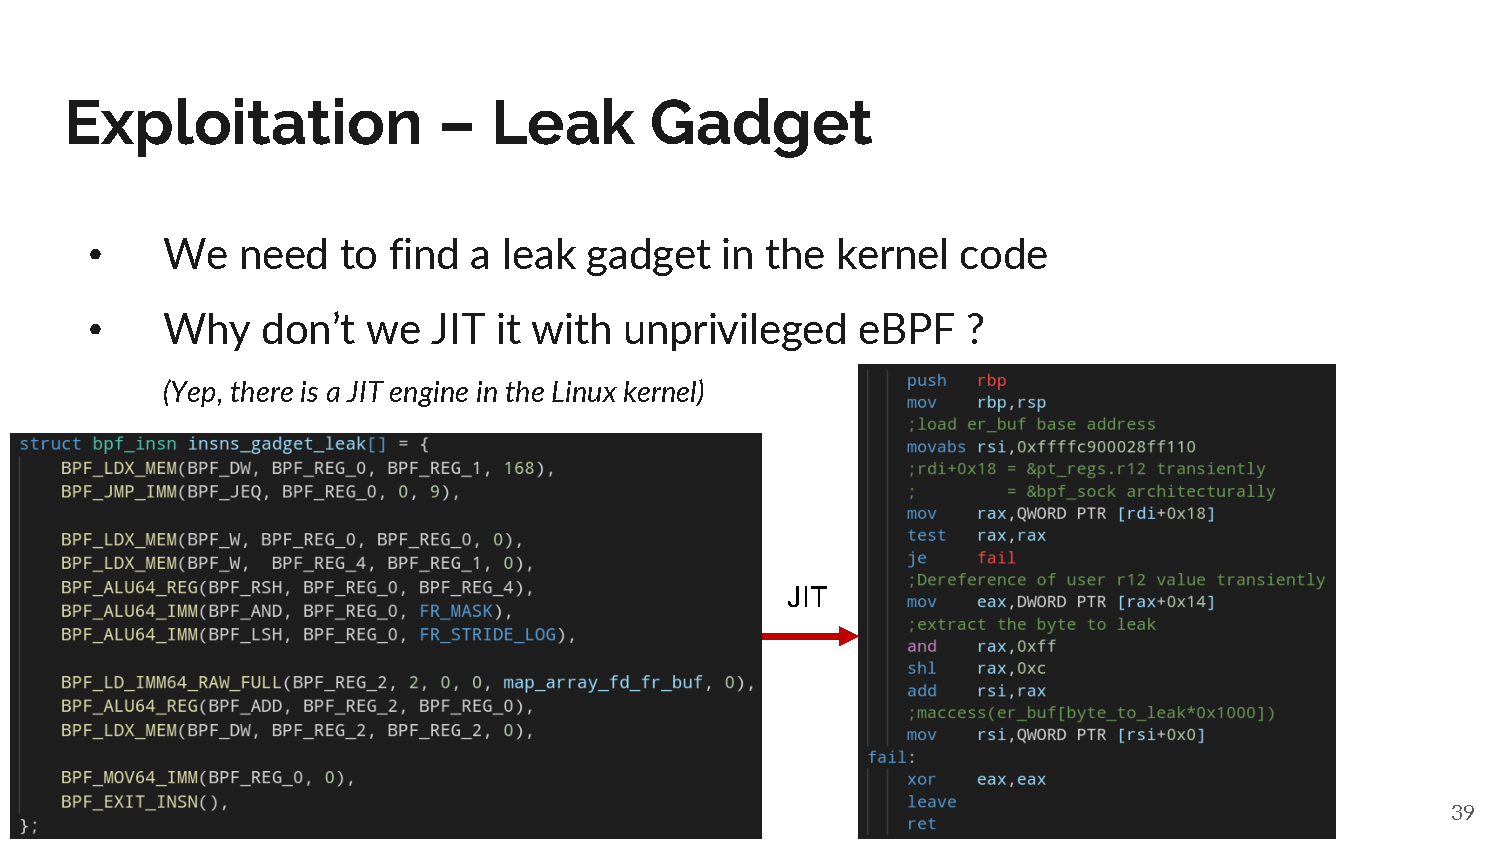
\includegraphics[width=1\textwidth]{img/ebpf.pdf}
        \end{center}
    \end{figure} 
\end{frame}

\begin{frame}{TIKTAG\cite{tiktag}}
    \begin{figure}
        \begin{center}
            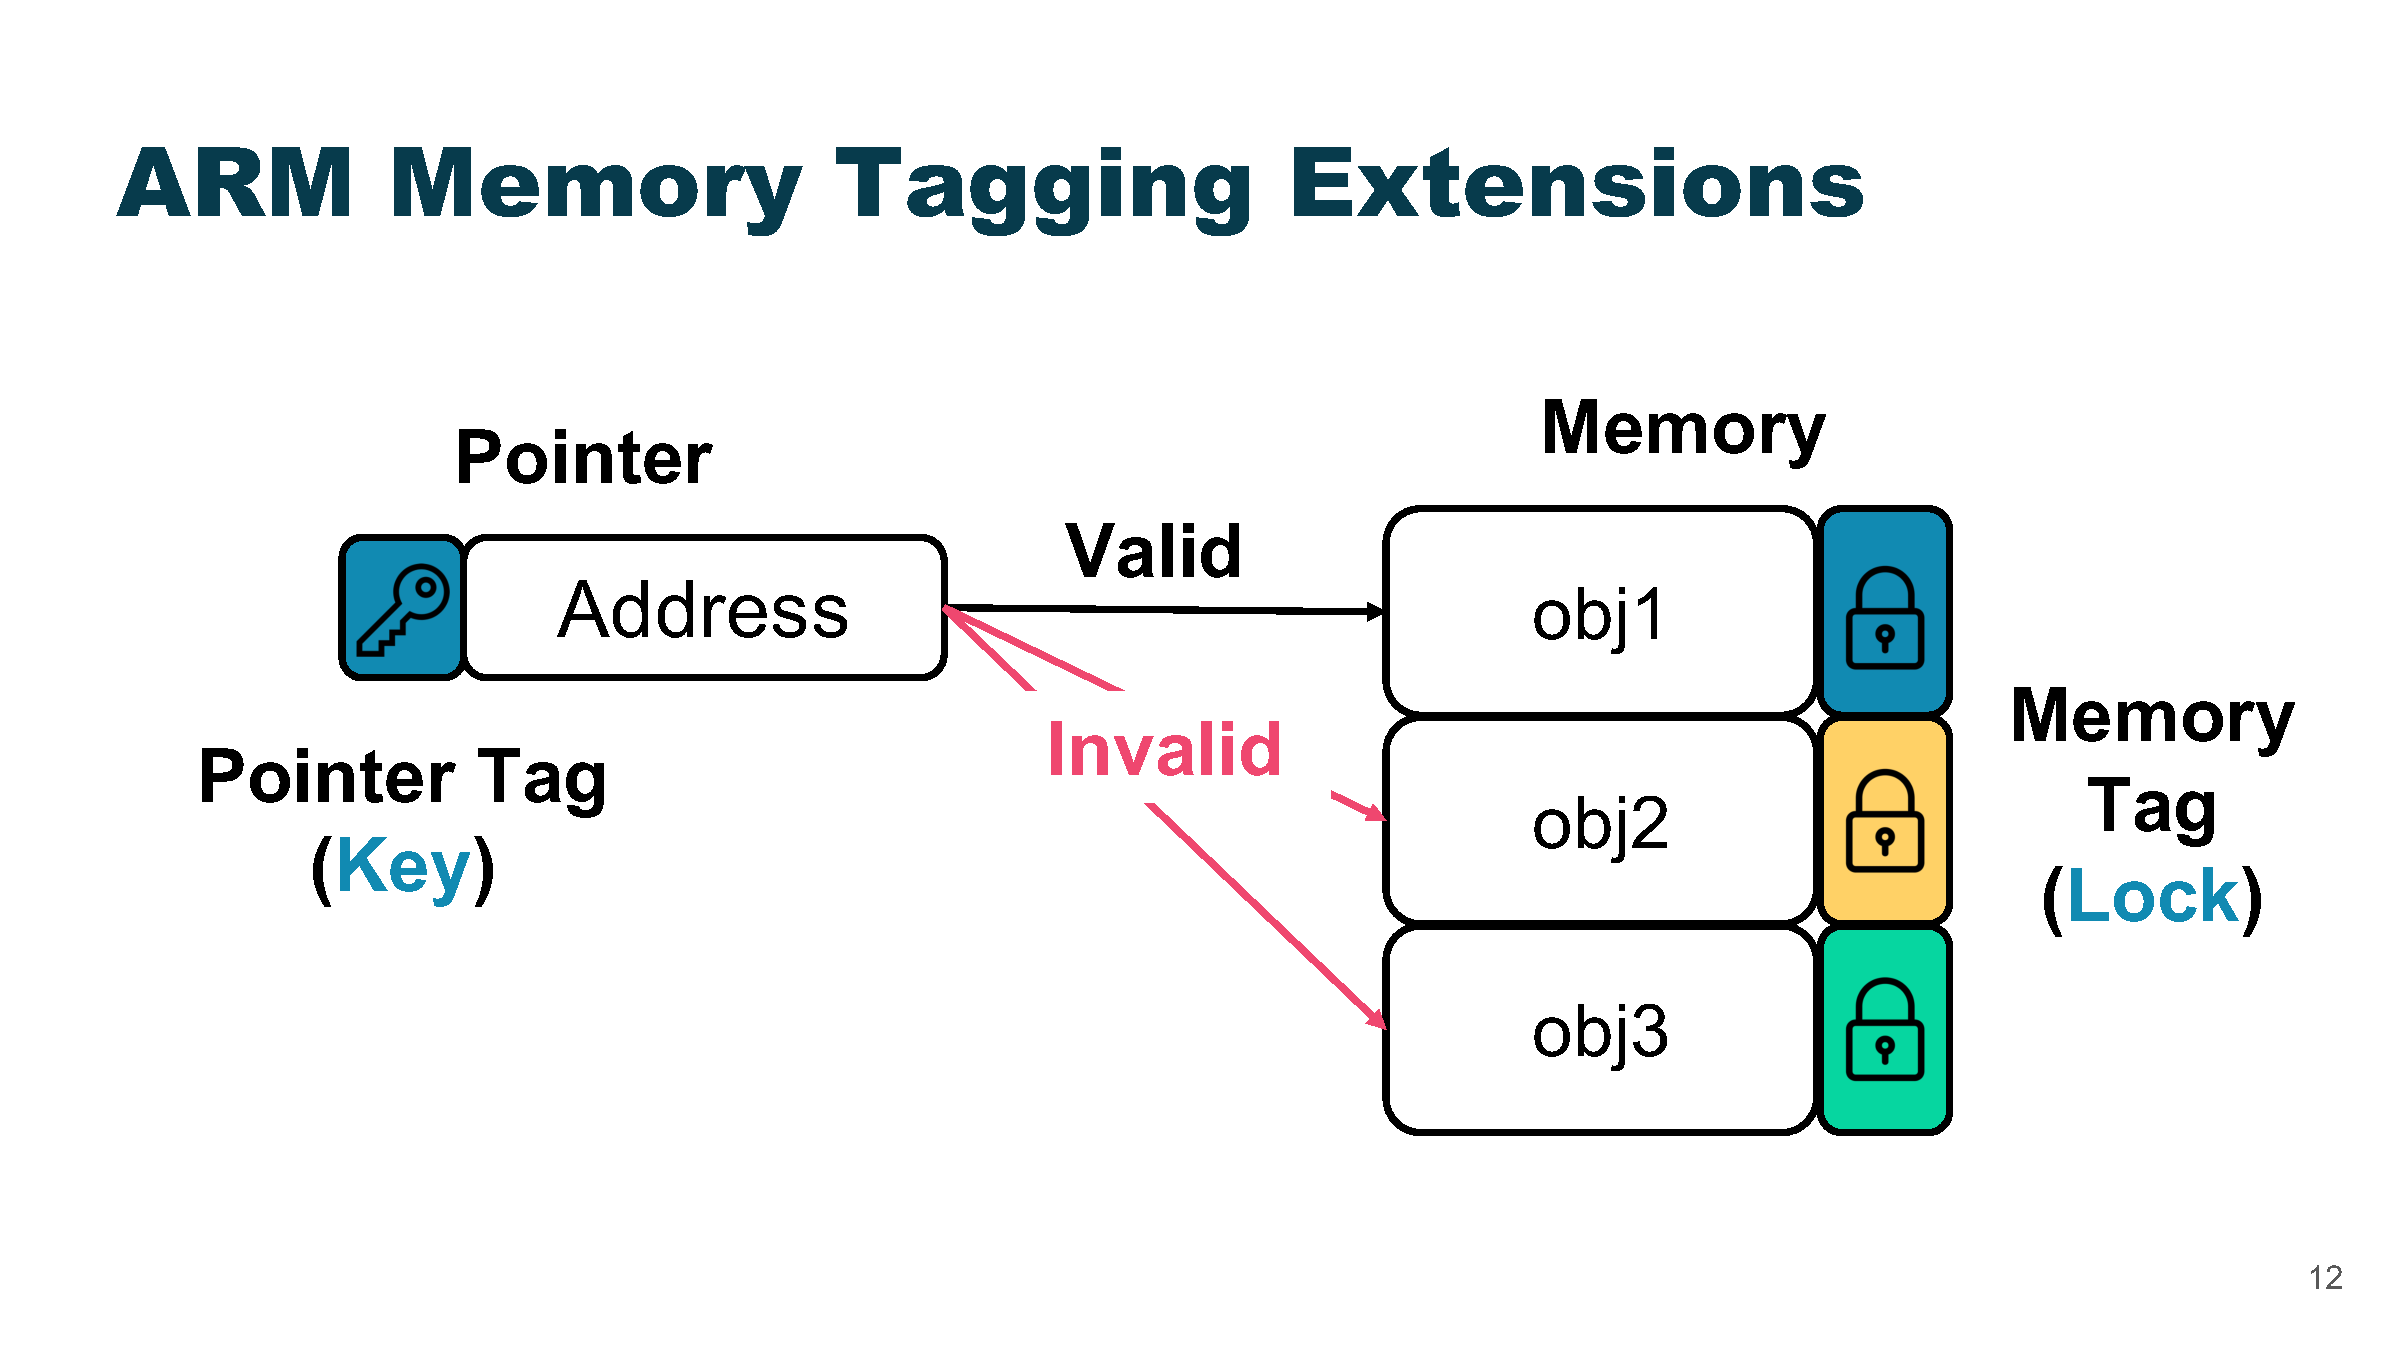
\includegraphics[width=1\textwidth]{img/mte.pdf}
        \end{center}
    \end{figure} 
\end{frame}

\begin{frame}{TIKTAG\cite{tiktag}}
    \begin{figure}
        \begin{center}
            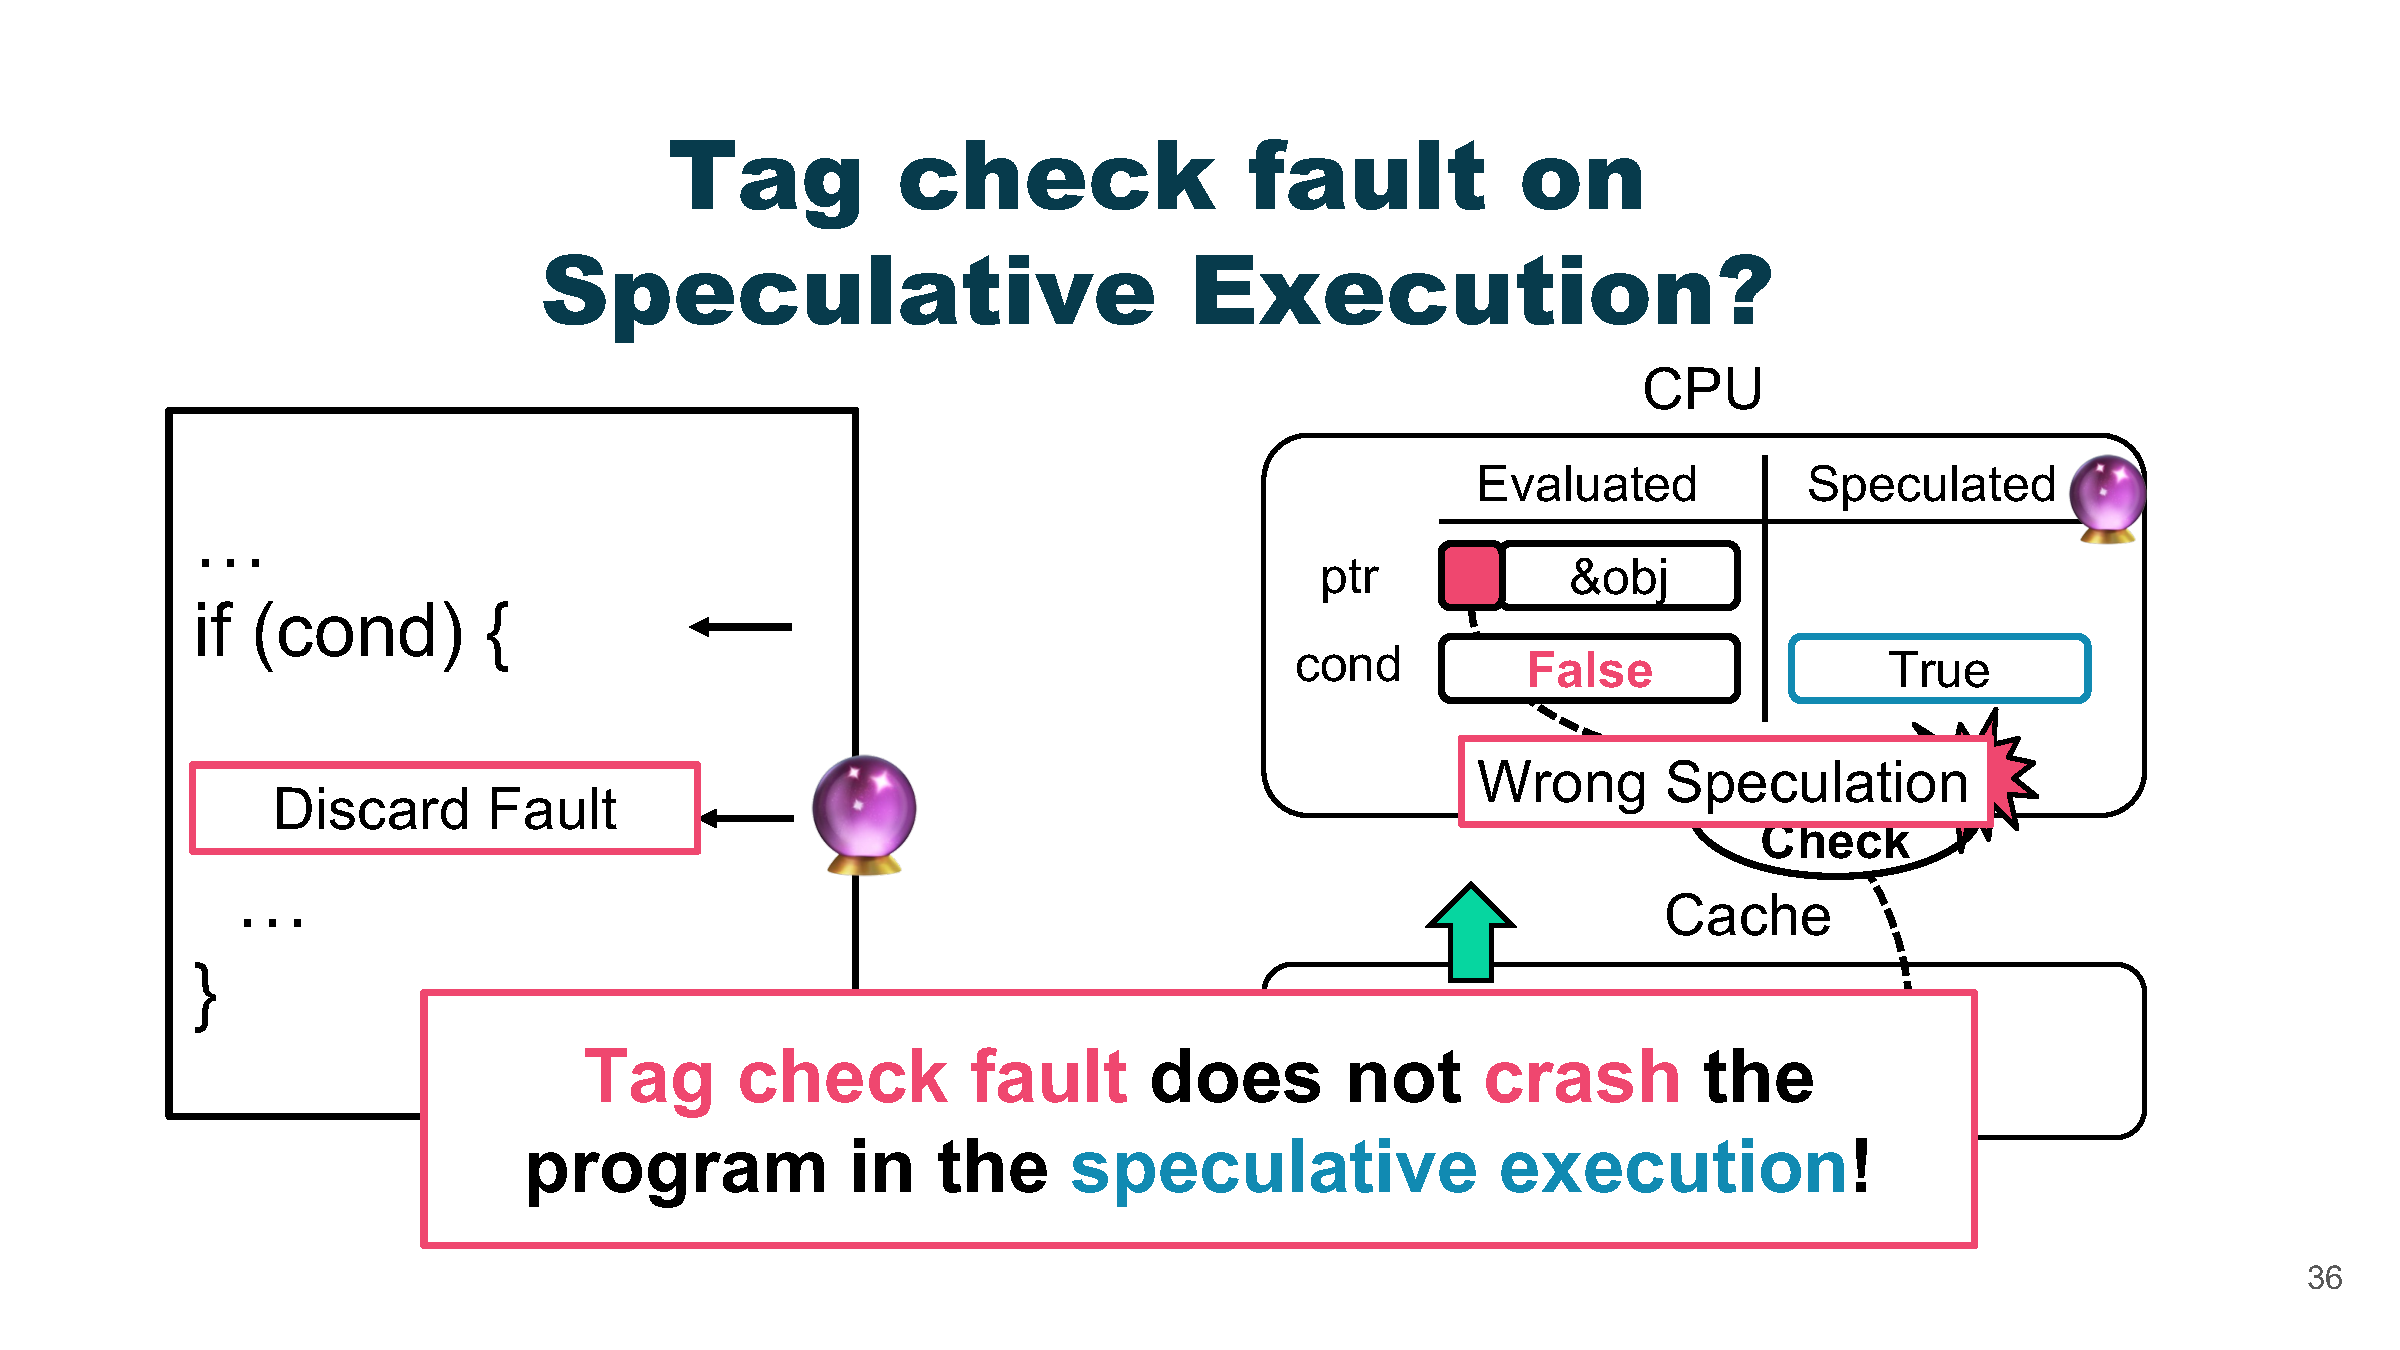
\includegraphics[width=1\textwidth]{img/tiktag.pdf}
        \end{center}
    \end{figure} 
\end{frame}

\begin{frame}{TIKTAG\cite{tiktag}}
    \begin{center}
        \Large
        Speculative prefetch of instructions \\
        $\Rightarrow$ \textbf{Avoid} segmentation fault to leak KASLR \\
    \end{center}
    \begin{center}
        \Large
        Exploit speculative execution \\
        $\Rightarrow$ \textbf{Bypass} memory tag check fault
    \end{center}
\end{frame}

\begin{frame}{TIKTAG\cite{tiktag}}
    \begin{figure}
        \begin{center}
            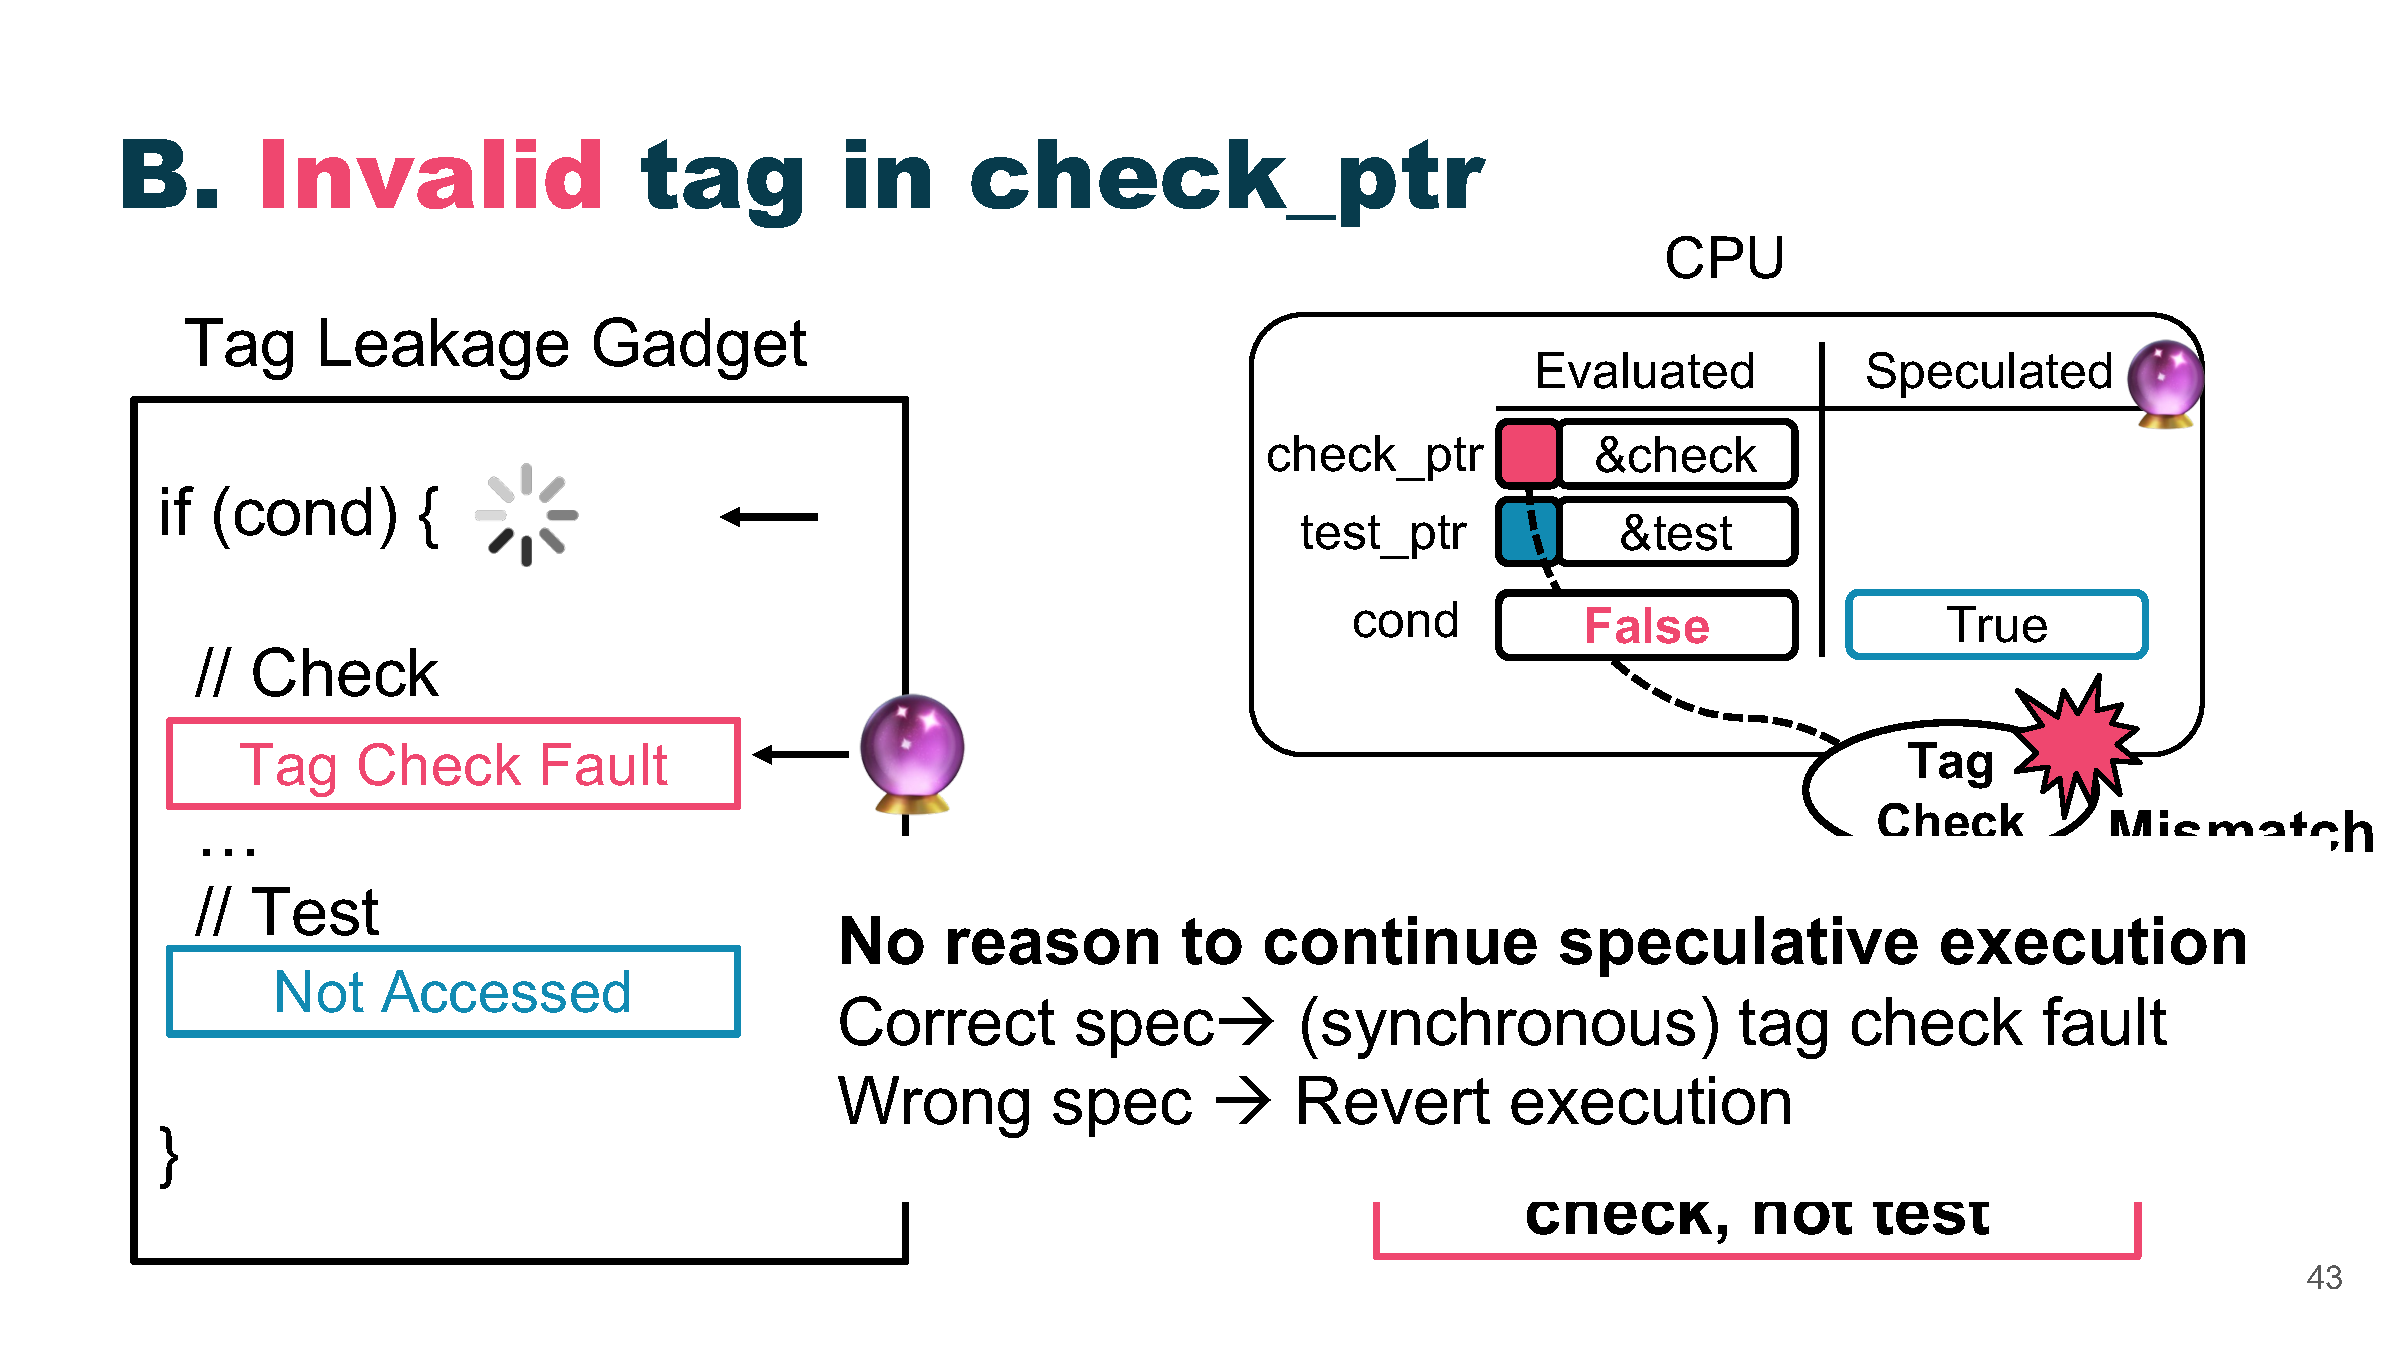
\includegraphics[width=1\textwidth]{img/mte-sc1.pdf}
        \end{center}
    \end{figure} 
\end{frame}

\begin{frame}{TIKTAG\cite{tiktag}}
    \begin{figure}
        \begin{center}
            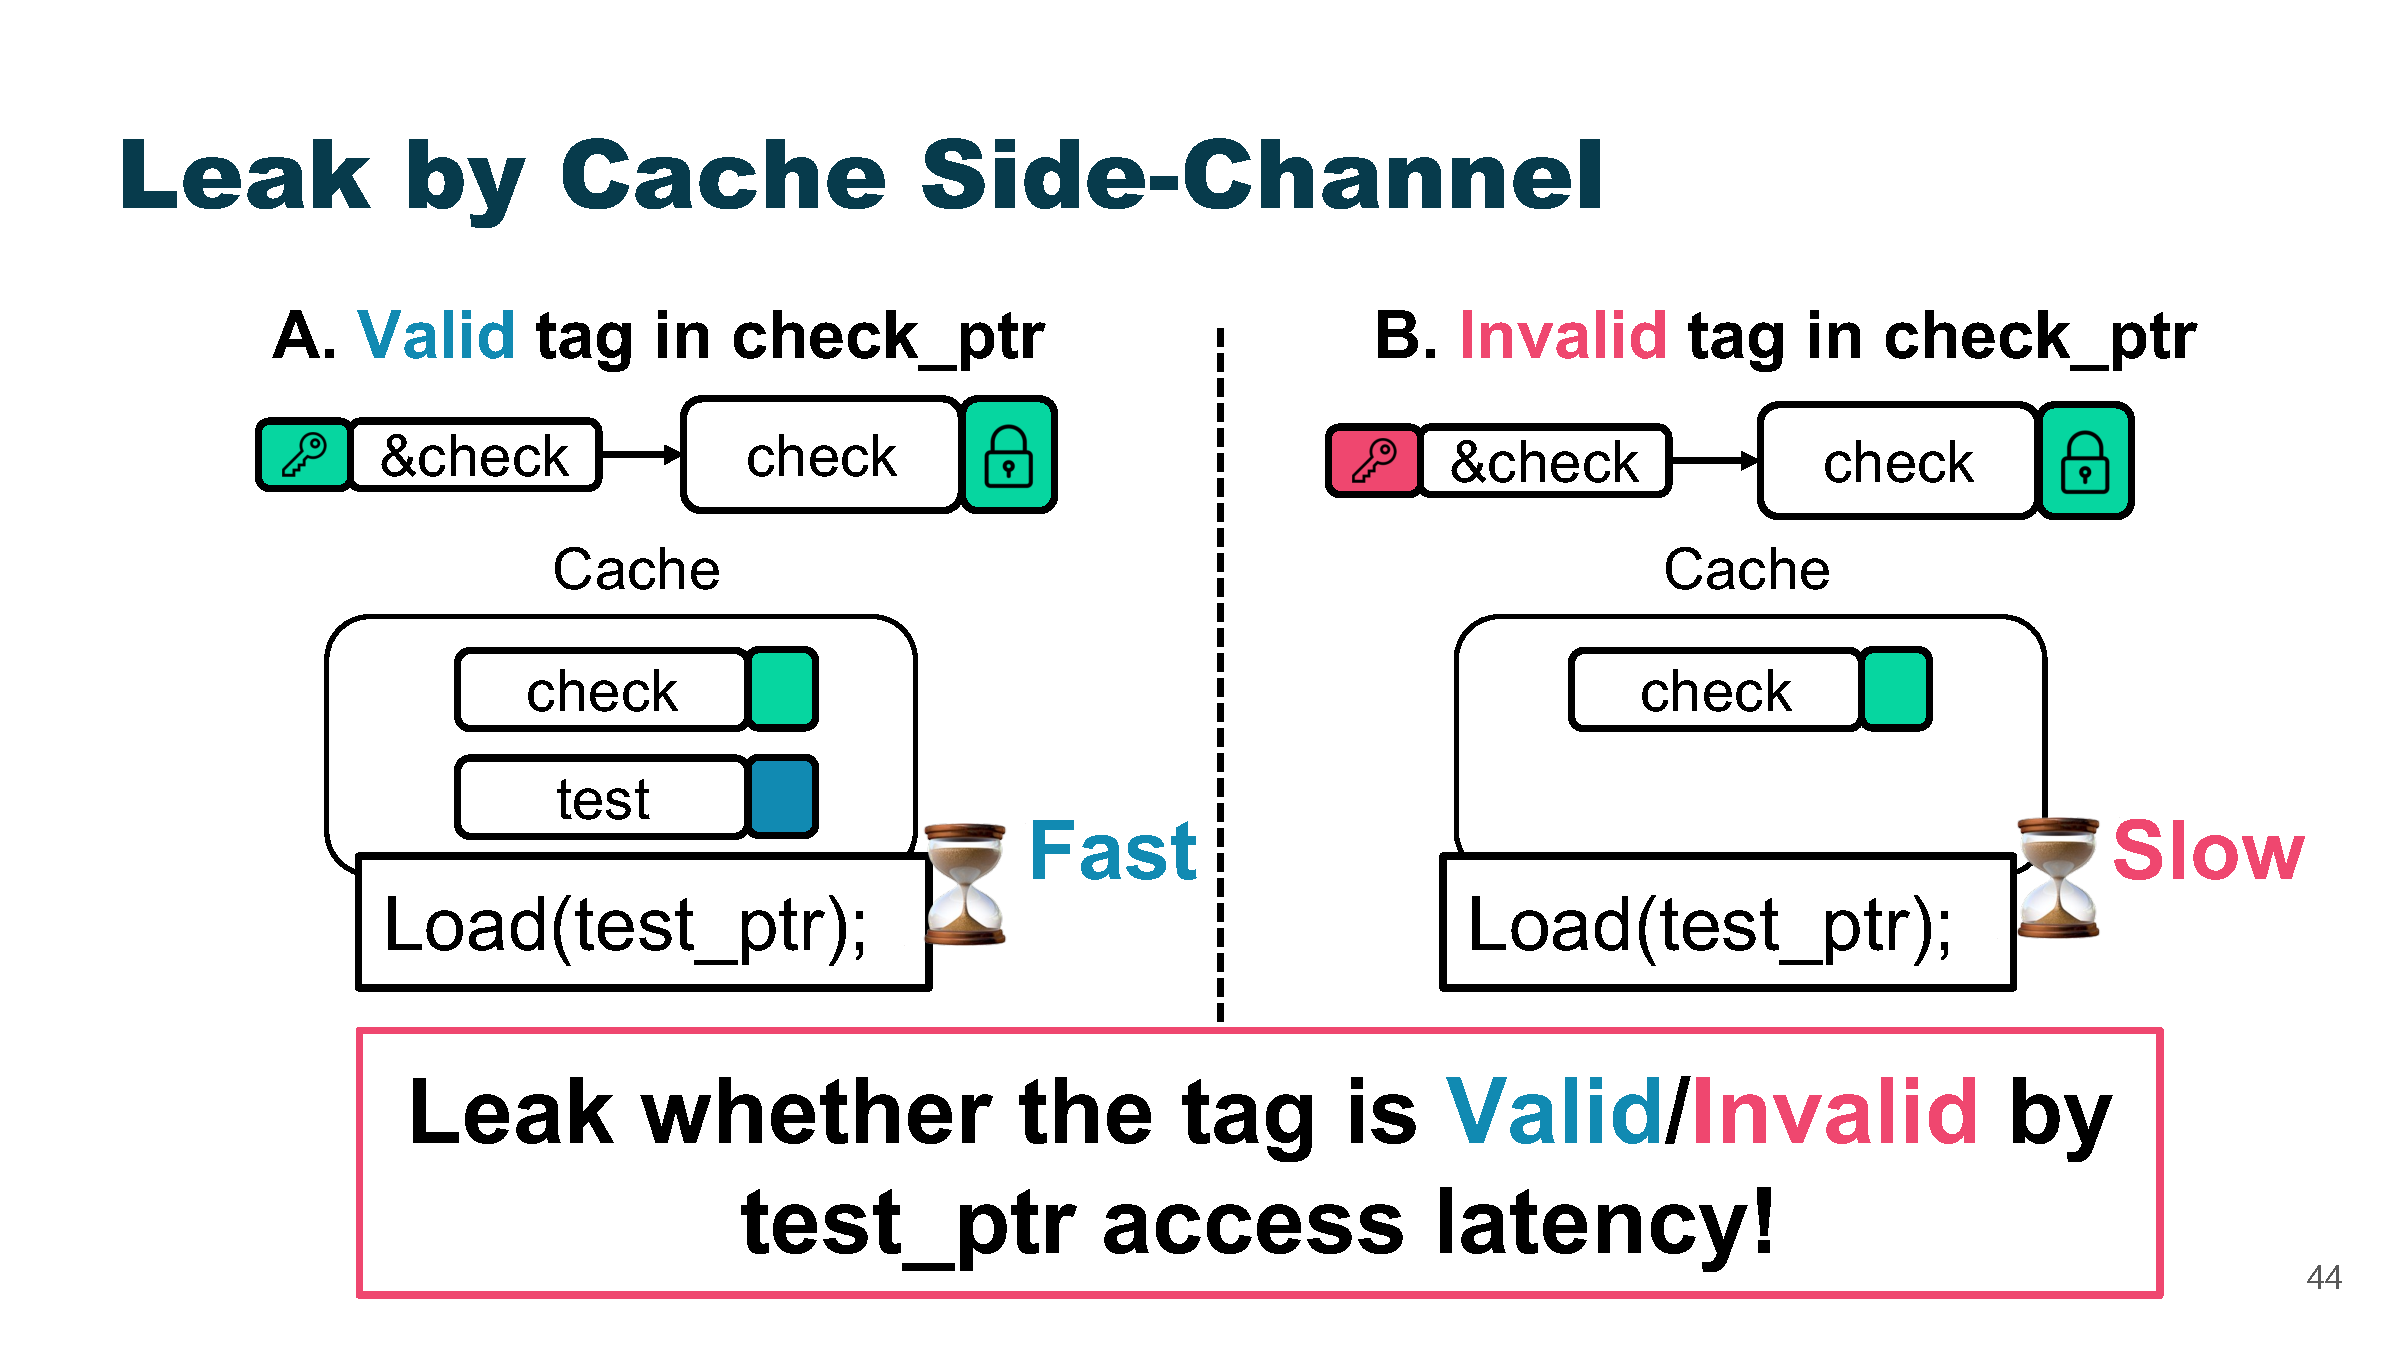
\includegraphics[width=1\textwidth]{img/mte-sc2.pdf}
        \end{center}
    \end{figure} 
\end{frame}

\begin{frame}{TIKTAG\cite{tiktag}}
    \begin{figure}
        \begin{center}
            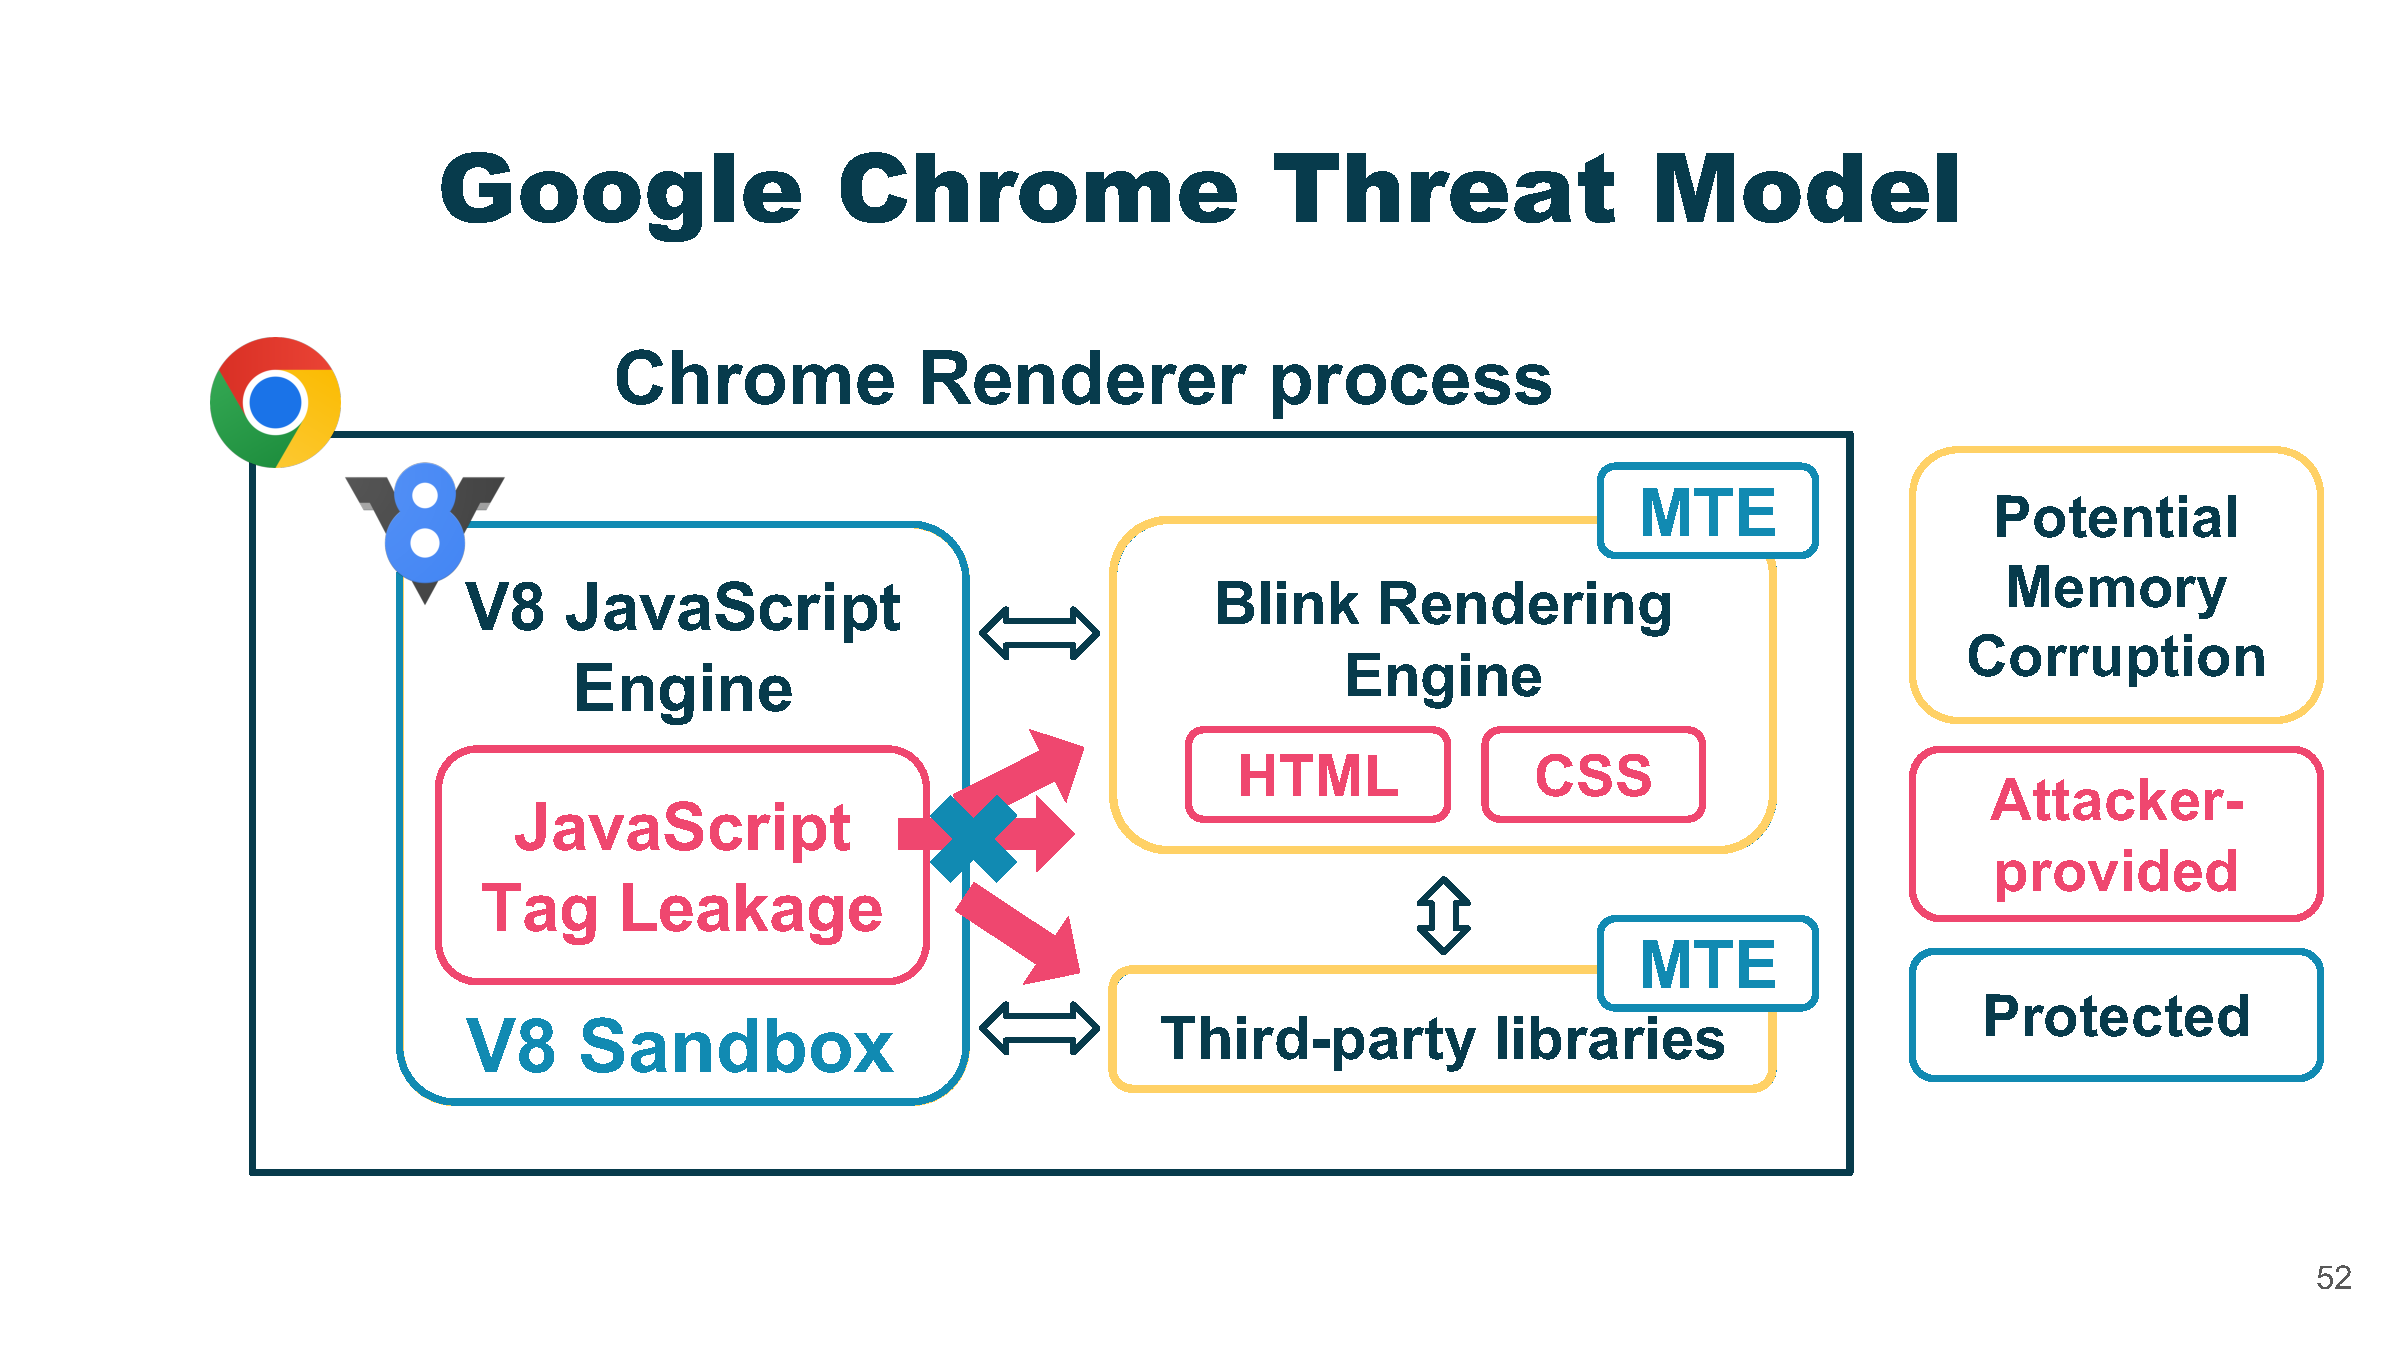
\includegraphics[width=1\textwidth]{img/chrome.pdf}
        \end{center}
    \end{figure} 
\end{frame}

\begin{frame}{TIKTAG\cite{tiktag}}
    Case Study: Chrome MTE Bypass Attack
    \begin{itemize}
        \item Leak MTE tag of vulnerable object
        \item Leak MTE tag of target object
        \item Keep reallocating target if the tags are different
        \item Access target object with forged pointer
    \end{itemize}
\end{frame}


\begin{frame}{TIKTAG\cite{tiktag}}
    \begin{figure}
        \begin{center}
            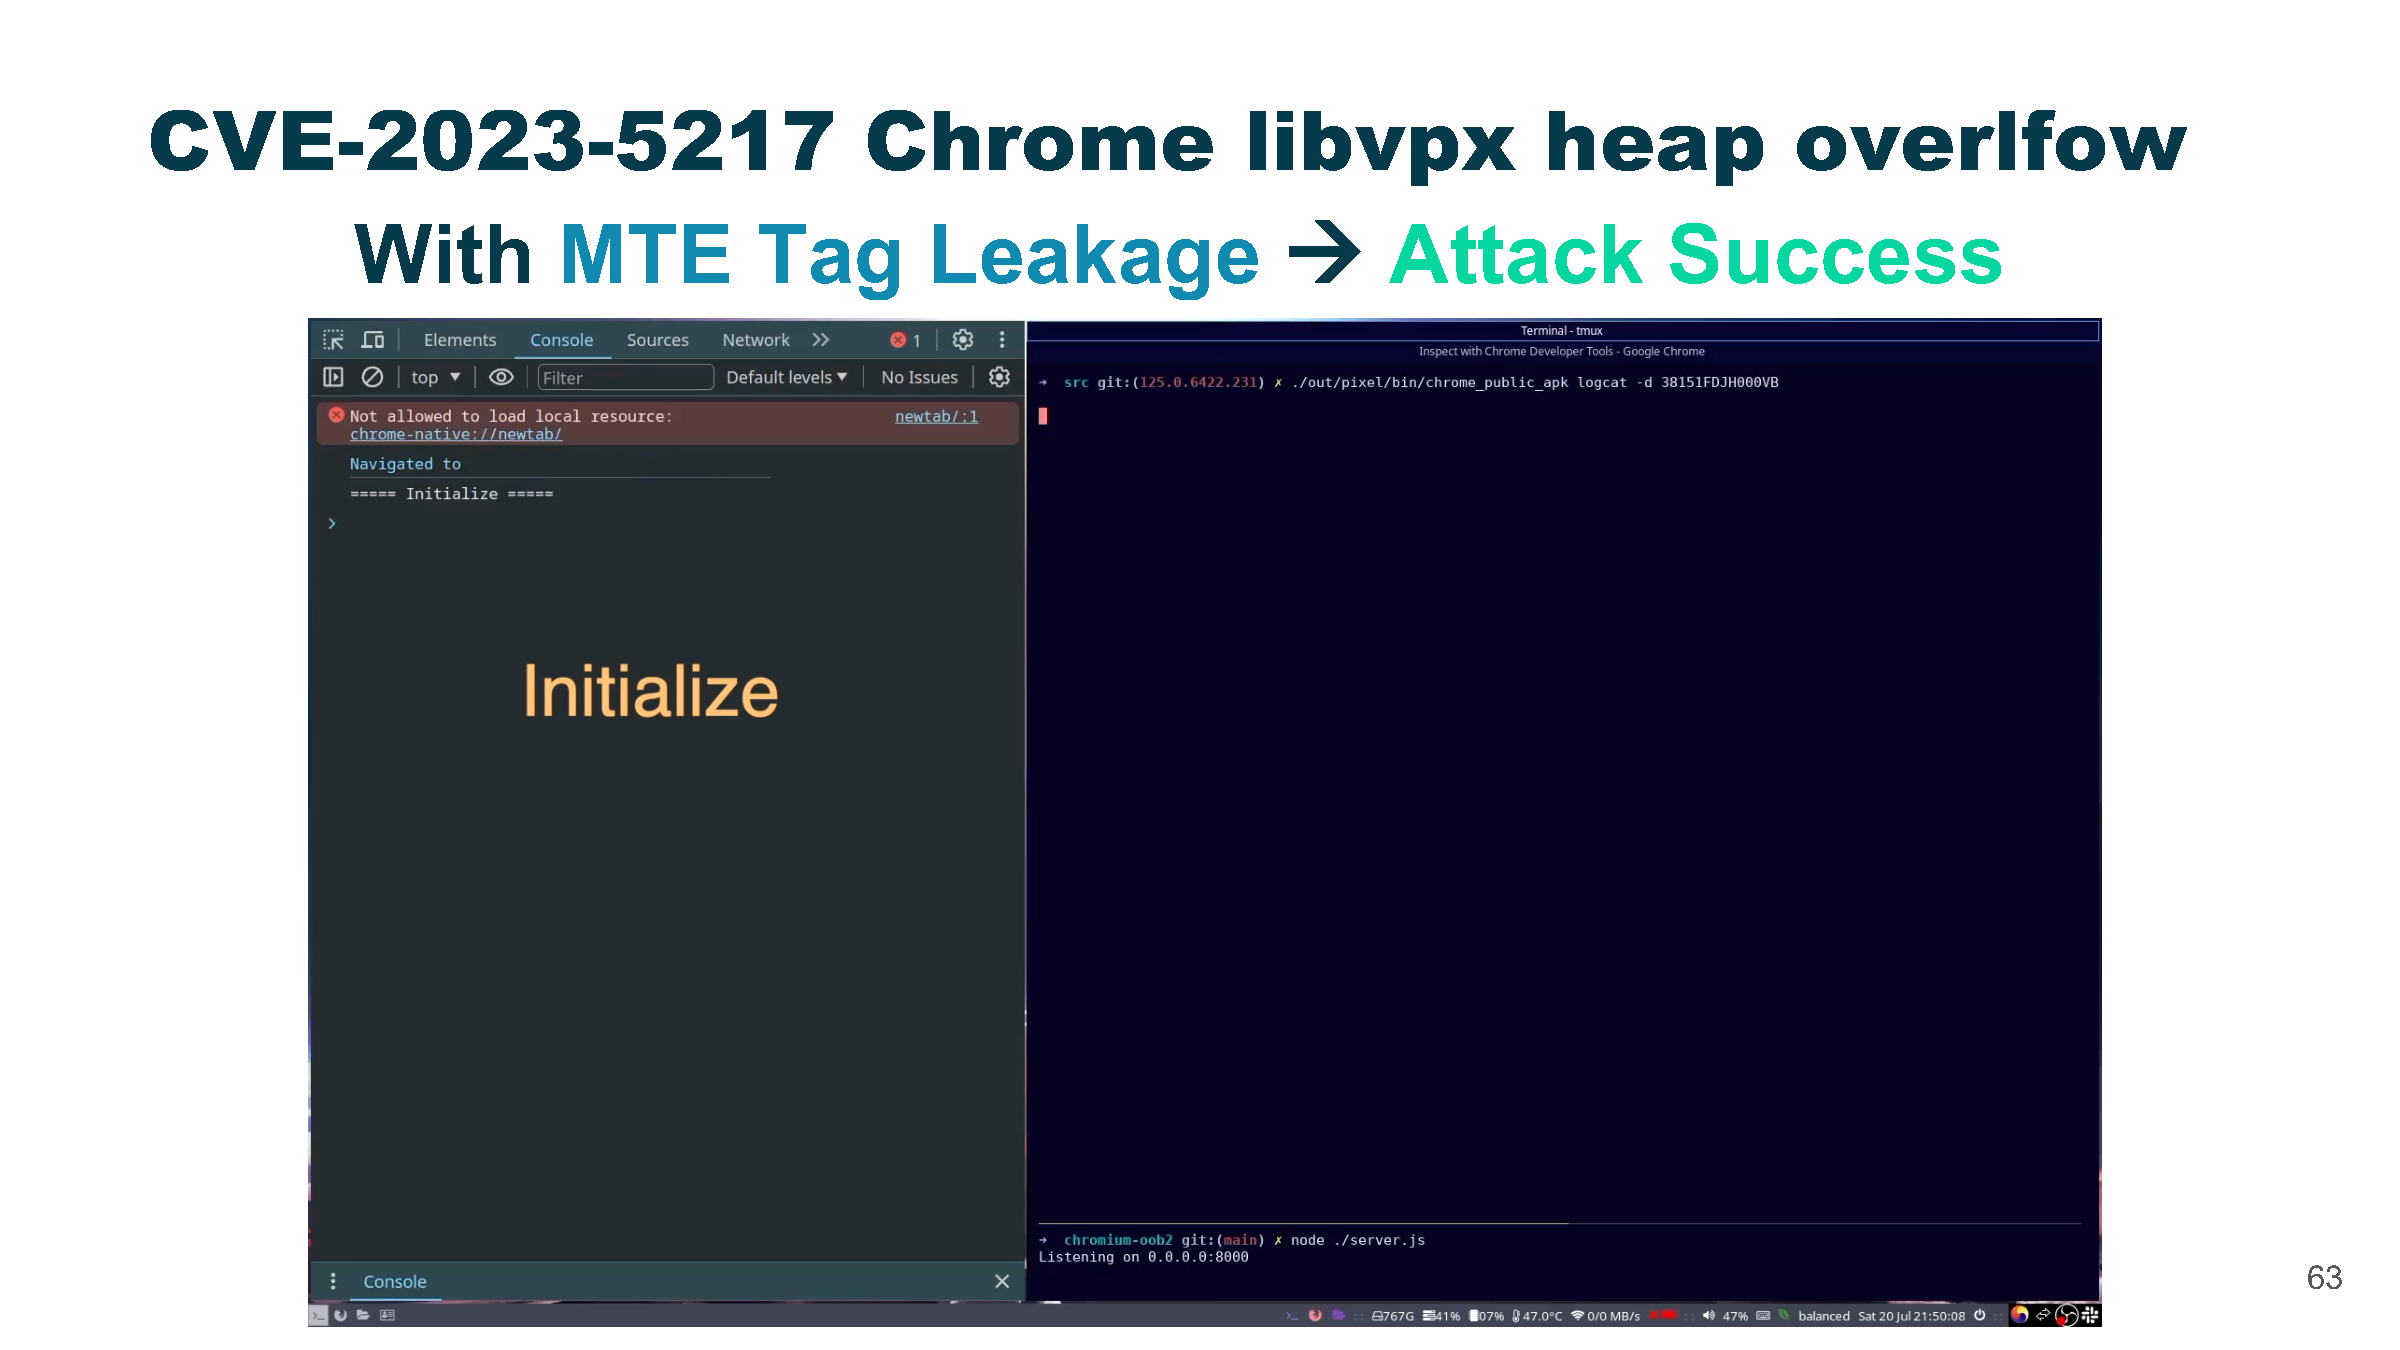
\includegraphics[width=1\textwidth]{img/cve.pdf}
        \end{center}
    \end{figure} 
\end{frame}

\begin{frame}{PACMAN\cite{pacman}}
    \begin{figure}
        \begin{center}
            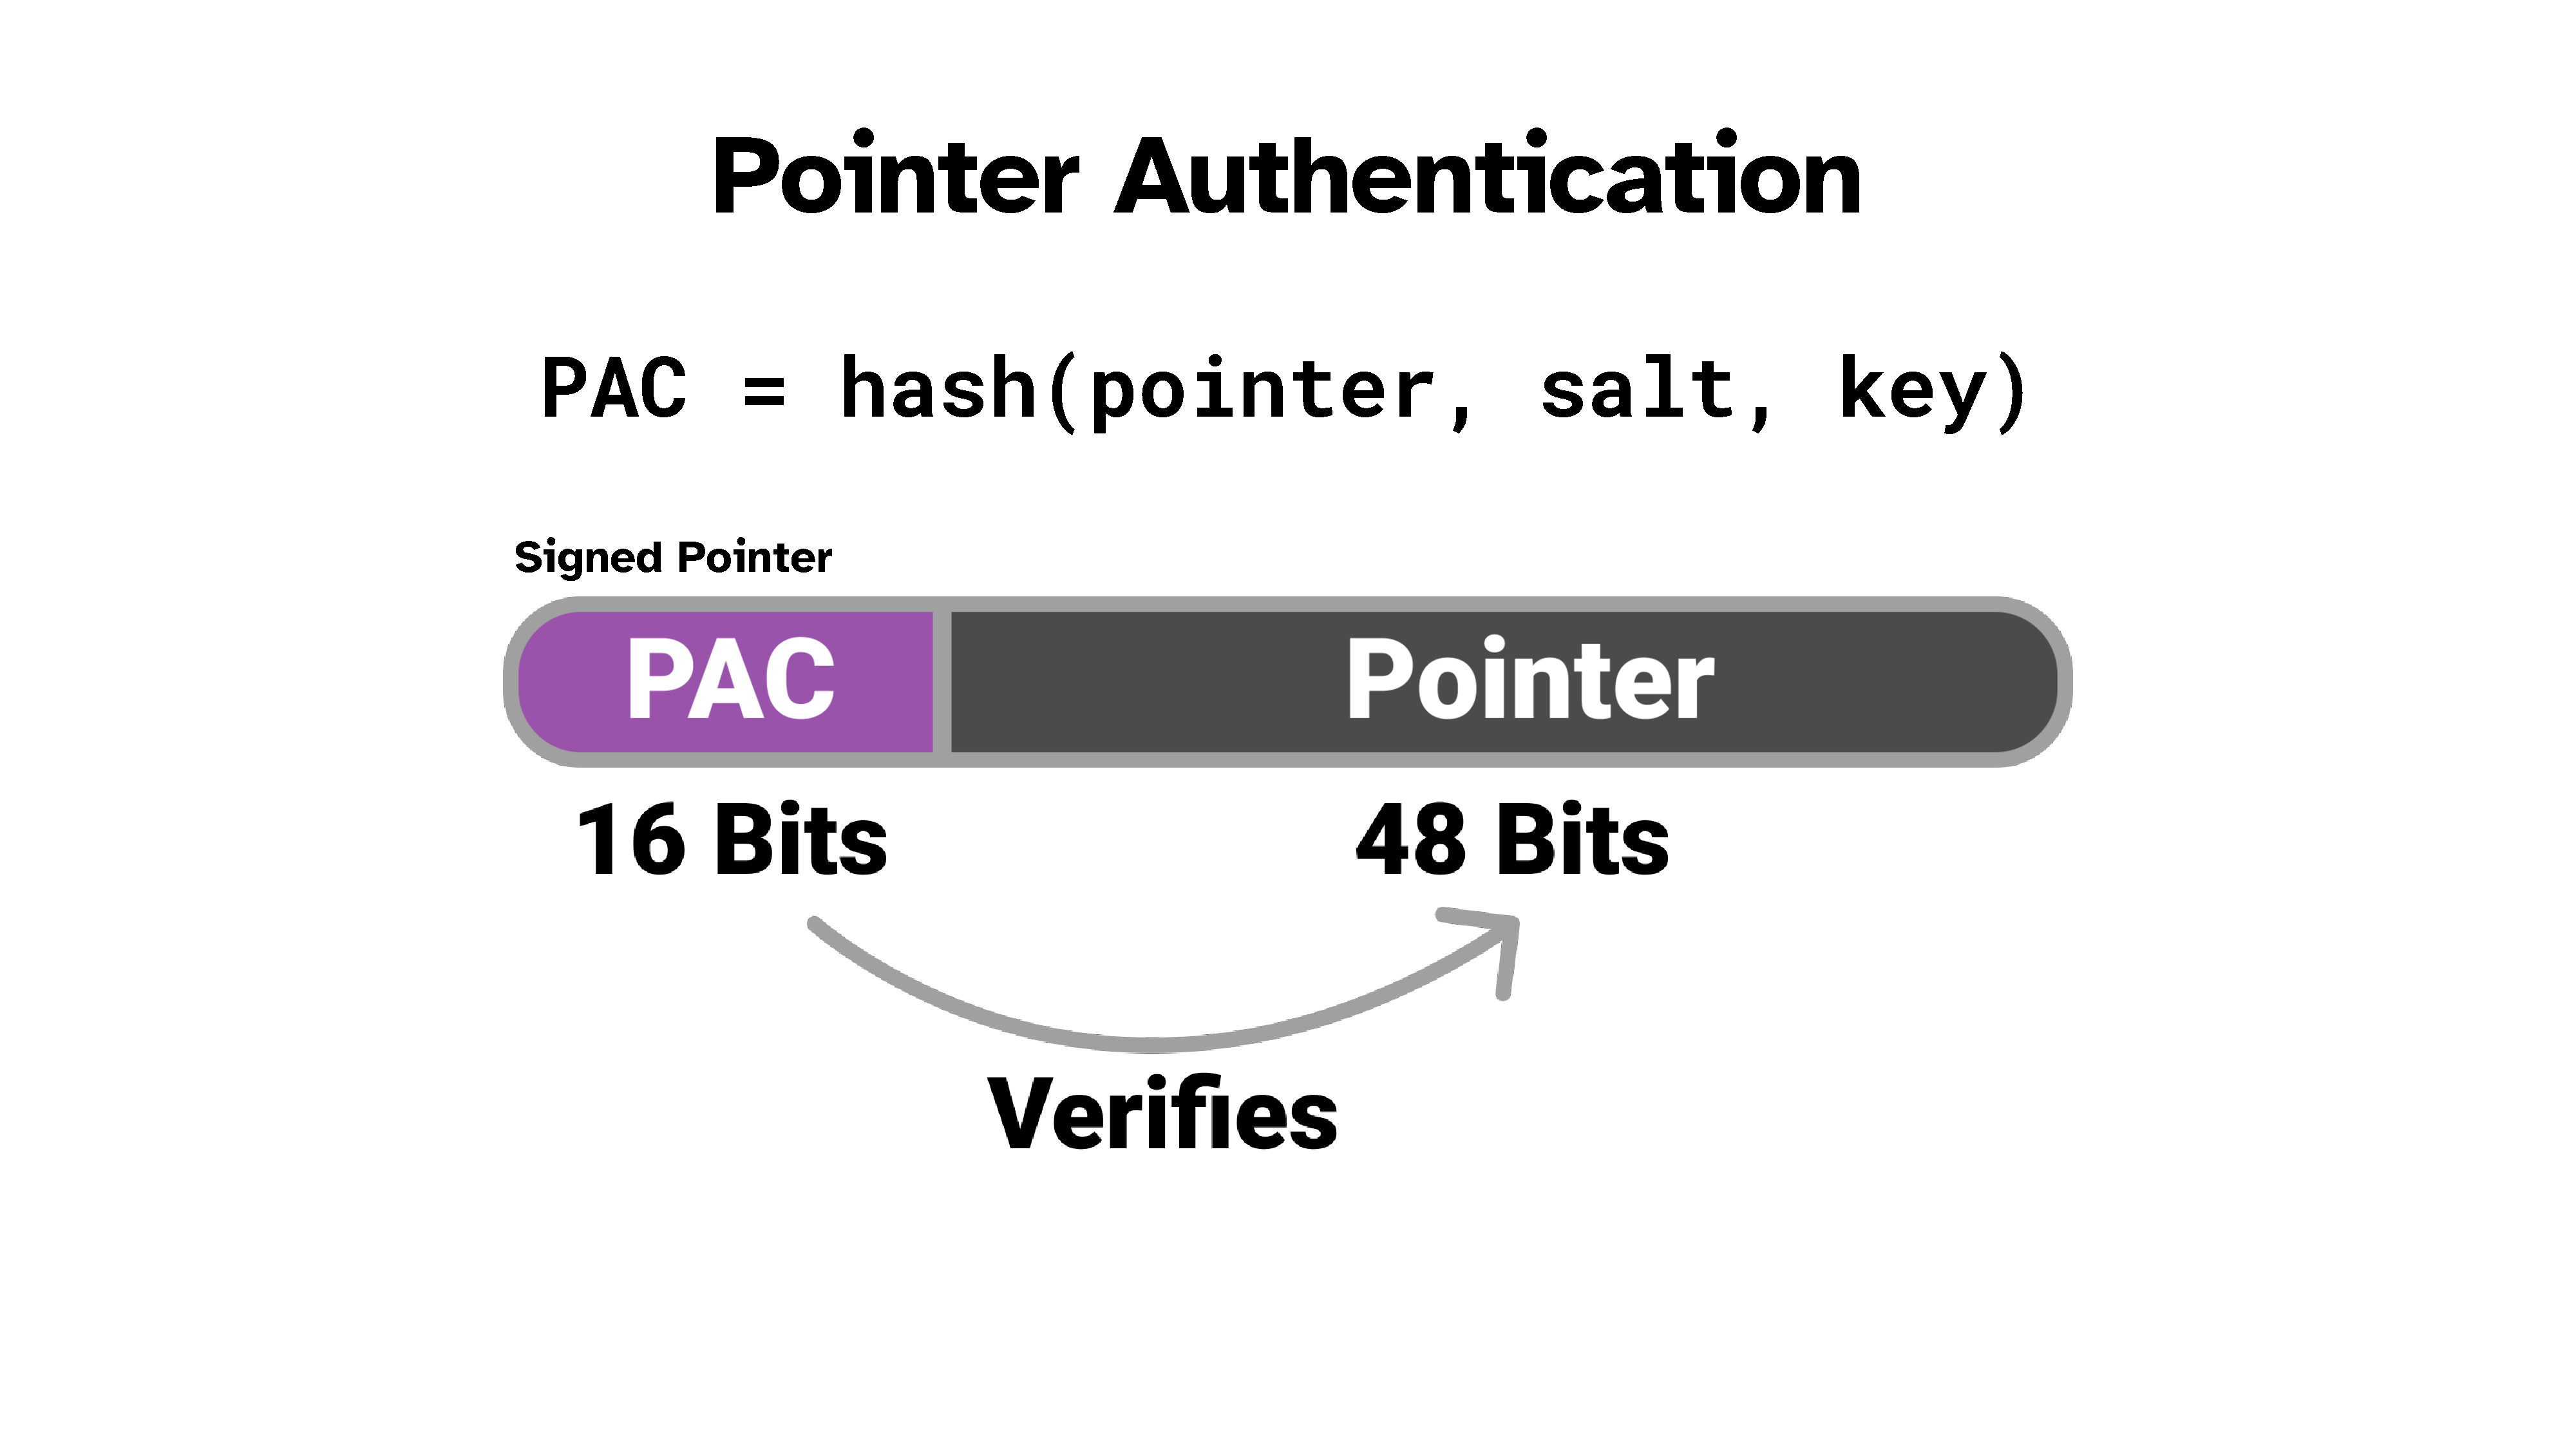
\includegraphics[width=1\textwidth]{img/pac.pdf}
        \end{center}
    \end{figure} 
\end{frame}

\begin{frame}{PACMAN\cite{pacman}}
    \begin{figure}
        \begin{center}
            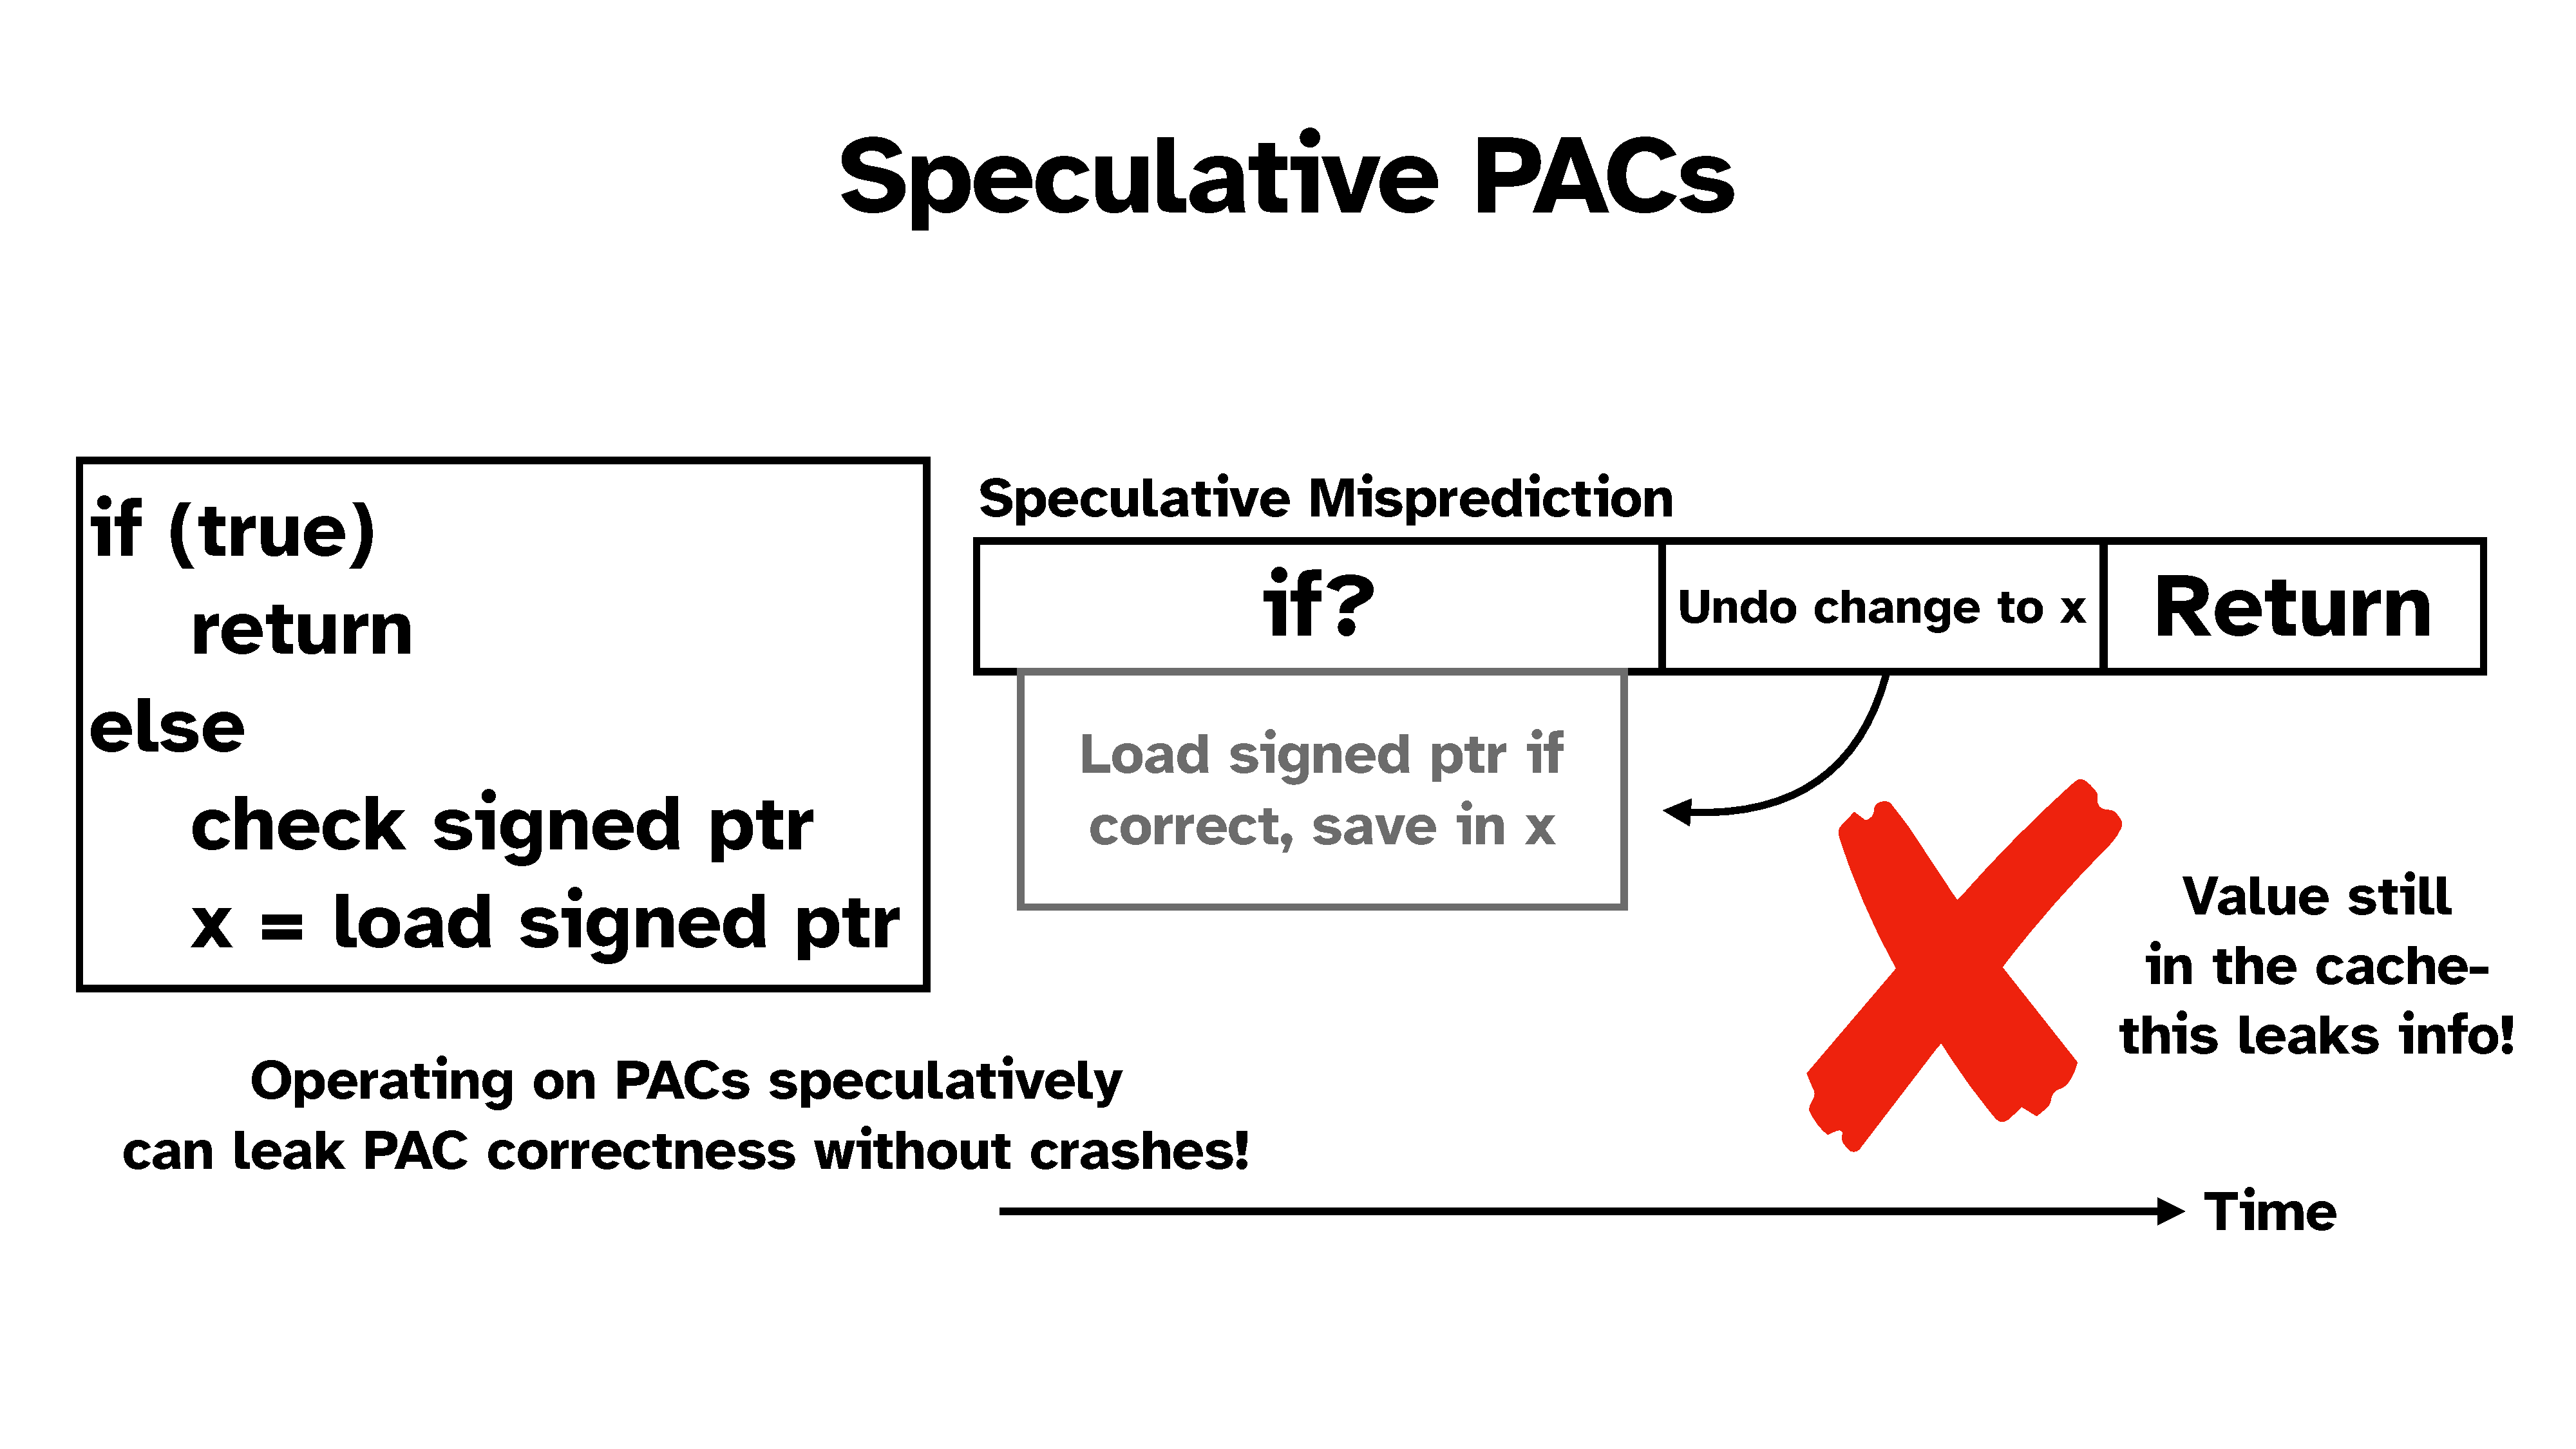
\includegraphics[width=1\textwidth]{img/pacman.pdf}
        \end{center}
    \end{figure} 
\end{frame}

\begin{frame}[allowframebreaks]{References}
\tiny
\printbibliography
\end{frame}
\end{document}
